\documentclass[12pt]{article}
\usepackage[utf8]{inputenc} %mogu sa ovim pisati ščđžć
\usepackage{extsizes} %mogu koristi visinu fonta koju želim 	%

%\usepackage{hyperref} 					
\usepackage{hhline}
\usepackage{tikz}
\usepackage{amsmath}
\usepackage{listings}
\usepackage{amsmath}
%\usepackage{xcolor}
\lstset { %
	language=C++,breaklines=true,showstringspaces=false,
	backgroundcolor=\color{black!5}, % set backgroundcolor
	keywordstyle=\color{red},
	commentstyle=\color{blue},
	basicstyle=\sffamily,% basic font setting
	numbers=left,%
	numberstyle={\tiny \color{black}},% size of the numbers
	numbersep=9pt, % this defines how far the numbers are from the text
}

\usepackage{times}

\usepackage{geometry} %štimanje margina
\geometry{textwidth=18cm}
\geometry{textheight=22cm}

\usepackage[english]{babel}

\usepackage{array} %za tabele
\newcolumntype{P}[1]{>{\centering\arraybackslash}p{#1}}

\usepackage{enumitem}

\usepackage{caption}
\usepackage{subcaption}

% \usepackage{tabu} % for thick lines in tables
\usepackage{makecell}
\usepackage{hhline}

\usepackage{multicol} % multikolone
\usepackage{graphicx}
\usepackage{setspace}

\usepackage[obeyspaces]{url} % for adding paths to a folder
\graphicspath{{./figures/}}

%\path{{./Data/}} % adddig a path to a folder

\usepackage{wrapfig} %wraps figure
\usepackage{lipsum}  %fills text around figure

\usepackage{bm}  %mogu pisati boldirane formule sa simbolima

\usepackage{amssymb} % za pisannje skupova

\usepackage[usestackEOL]{stackengine} %za piasanje front page-a
\numberwithin{equation}{section}

%\makeatletter
%\renewcommand{\@seccntformat}[1]{}
%\makeatother  % removes numbers from sections but keeps the references
\usepackage{fancyhdr}
\pagestyle{fancy}
\fancyhf{}
\rhead{\scriptsize \hspace*{0cm}  Thesis topic: Graph-Based Keyword Extraction from
 \\ Scientific Paper Abstracts using Word Embeddings}
\lhead{\scriptsize Universit\`a  di Bologna \\ Department of Computer Science and Engineering}
\fancyheadoffset{1cm} % to offset the header by some distance 


\usepackage{epsfig}
\usepackage{multirow}
\usepackage{pdfpages}
\setcounter{MaxMatrixCols}{20} % maksimalan broj kolona na 20
\usepackage{float} % da slike nisu poremećene
\usepackage[figurename=Figure]{caption} % mijenja ime sa figure u slika
\usepackage[tablename=Table]{caption} % mijenja ime sa figure u slika

\usepackage{chngcntr}
%\counterwithout{figure}{chapter} % stavlja bojeve unutar captiona slike

\usepackage{colortbl} % color in tables

\addto\captionsenglish{% Replace "english" with the language you use
	\renewcommand{\contentsname}% Promjena naziva content
	{Content}%
}

\usepackage{etoolbox}
%\patchcmd{\thebibliography}{\section*{\refname}}{}{}{} % smakinje ime references

%\usepackage[colorlinks=true, linkcolor = cyan]{hyperref}
\usepackage{hyperref}

%rotating picture
\usepackage{lscape}
\usepackage{rotating}

% tilda
\usepackage{undertilde}

%%coloring links
%\usepackage{hyperref}
%\hypersetup{
	%	colorlinks = true,
	%	linkbordercolor = [white],
	%	linkcolor = [magenta]
	%}

%\usepackage[colorlinks]{hyperref}
%\hypersetup{colorlinks=true, linkcolor=cyan,linkbordercolor=red}

%matlab
\usepackage{listings}
\usepackage{color} %red, green, blue, yellow, cyan, magenta, black, white
\definecolor{mygreen}{RGB}{28,172,0} % color values Red, Green, Blue
\definecolor{mylilas}{RGB}{170,55,241}


\lstset{
	language=Matlab,
	basicstyle=\footnotesize\ttfamily,
	breaklines=true,%
	morekeywords={matlab2tikz},
	keywordstyle=\color{blue},%
	morekeywords=[2]{1}, keywordstyle=[2]{\color{black}},
	identifierstyle=\color{black},%
	stringstyle=\color{mylilas},
	commentstyle=\color{mygreen},%
	showstringspaces=false,%without this there will be a symbol in the places where there is a space
	numbers=left,%
	numberstyle={\tiny \color{black}},% size of the numbers
	numbersep=9pt, % this defines how far the numbers are from the text
	emph=[1]{for,end,break},emphstyle=[1]\color{red}, %some words to emphasise
	emph=[2]{word1,word2}, emphstyle=[2]{style},   
}

\addto\captionsenglish{% Replace "english" with the language you use
	\renewcommand{\contentsname}% Promjena naziva content
	{Contents}%
}

% stil numerisanja stranica
\usepackage{lastpage}
\cfoot{Page \thepage \hspace{1pt} of \pageref{LastPage}}

\usepackage{etoolbox}
\patchcmd{\thebibliography}{\section*{\refname}}{}{}{} % smakne ime references

% za pisanje pseudokoda
\usepackage[plain]{algorithm2e}
%\usepackage{algorithmic}
%\usepackage{algpseudocode}
%\usepackage{algorithmicx}
%\usepackage{algorithm}
%\usepackage{algpseudocode}
%\algnewcommand\algorithmicinput{\textbf{Function:}}
%\algnewcommand\Function{\item[\algorithmicinput]}
%\usepackage{capt-of}
\SetAlgorithmName{Pseudocode}

%\renewcommand{\@algocf@capt@plain}{top}% formerly {bottom}

\makeatletter
\newenvironment{breakablealgorithm}
{% \begin{breakablealgorithm}
		\begin{center}
			\refstepcounter{algorithm}% New algorithm
			\hrule height.8pt depth0pt \kern2pt% \@fs@pre for \@fs@ruled
			\renewcommand{\caption}[2][\relax]{% Make a new \caption
				{\raggedright\textbf{\fname@algorithm~\thealgorithm} ##2\par}%
				\ifx\relax##1\relax % #1 is \relax
				\addcontentsline{loa}{algorithm}{\protect\numberline{\thealgorithm}##2}%
				\else % #1 is not \relax
				\addcontentsline{loa}{algorithm}{\protect\numberline{\thealgorithm}##1}%
				\fi
				\kern2pt\hrule\kern2pt
			}
		}{% \end{breakablealgorithm}
		\kern2pt\hrule\relax% \@fs@post for \@fs@ruled
	\end{center}
}
\makeatother

\makeatletter
\newenvironment{breakalgo}[2][alg:\thealgorithm]{%
	\def\@fs@cfont{\bfseries}%
	\let\@fs@capt\relax%
	\par\noindent%
	\medskip%
	\rule{\linewidth}{.8pt}%
	\vspace{-3pt}%
	\captionof{algorithm}{#2}\label{#1}%
	\vspace{-1.7\baselineskip}%
	\noindent\rule{\linewidth}{.4pt}%
	\vspace{-1.3\baselineskip}%
}{%
	\vspace{-.75\baselineskip}%
	\rule{\linewidth}{.4pt}%
	\medskip%
}
\makeatother


\captionsetup{font=small}
\newcommand*{\matlab}{\textsc{Matlab}}
\newcommand*{\altmatlab}{{\mdseries\matlab}} 

\usepackage{xcolor}

\newsavebox{\bmatrixbox}
\newenvironment{colorbmatrix}
{\begin{lrbox}{\bmatrixbox}
		\mathsurround=0pt
		$\displaystyle
		\begin{bmatrix}}
		{\end{bmatrix}$%
	\end{lrbox}%
	\usebox{\bmatrixbox}%
	\kern-\wd\bmatrixbox
	\makebox[0pt][l]{$\left[\vphantom{\usebox{\bmatrixbox}}\right.$}%
	\kern\wd\bmatrixbox
}

\usepackage [autostyle, english = american]{csquotes}
\MakeOuterQuote{"}


\begin{document}
	
	\begin{titlepage}
		\begin{center}
			
			{\Large ALMA MATER STUDIORUM \\ UNIVERSIT\`A  DI BOLOGNA \\}
			\vspace{0.4cm} 
			\hrule
			\vspace{0.4cm} 
			{\Large DEPARTMENT OF COMPUTER SCIENCE AND ENGINEERING \\} 
			{\Large ARTIFICIAL INTELLIGENCE \\}
			\vspace{0.4cm} 
			\hrule
			\vspace{1cm}
			{\Large MASTER THESIS}\\[0.4cm]
			{\large in} \\[0.4cm]
			{\Large Natural Language Processing}\\[1cm]
			
			\hrule
			\vspace{0.4cm}
			
			{\Huge Graph-Based Keyword Extraction from}\\[0.3cm]
			{\Huge Scientific Paper Abstracts using Word Embeddings}
			\vspace{0.4cm}
			
			\hrule
			\vspace{2cm}
			
			{\large Author:}\\
			{\large Dinno Koluh\\}
			
			\vspace{2cm}
			
			{\large Supervisor:}\\[0.1cm]
			{\large Prof. Paolo Torroni}\\[0.4cm]
			
			{\large Co-Supervisor:}\\[0.1cm]
			{\large Dr. Federico Ruggeri}
			
			\vspace{2cm} 
			{\large Bologna,}\\[0.1cm] 
			{\large December 2023.}
			
		\end{center}
	\end{titlepage}
	\newpage
	\newgeometry{textwidth=16cm, textheight=22cm}
	\thispagestyle{empty}
	
	\begin{spacing}{1.5}
	\section*{Abstract}
	In the era of information overload it is essential to efficiently extract concise, precise and quality information from large texts. One aspect of information extraction is keyword extraction where large texts are represented as sets of keywords. This prospect of keyword extraction is paramount to researchers as they deal with huge numbers of scientific papers, and having a good and concise representation of those papers is essential for them. This thesis addresses that problem in the realm of Natural Language Processing (NLP). \\
	Using core NLP concepts and modeling texts as graphs, we are going to build a model for the automatic extraction of keywords. This is done in an unsupervised manner as the importance of a word is calculated through the position and weights associated with respective words in the graph. The first metric used to calculate the graph weights are co-occurrence matrices and the other metric are word embeddings. Word embeddings became a crucial way of representing the semantic information of words as dense vectors. \\
	The results of this paper were compared with keywords that were provided by authors of scientific papers in the area of computer science which act as the ground truth, but crucially are not a component in the model construction, but just serve as a verifier of the model's accuracy.
	
	\textbf{Keywords}: NLP, keyword extraction, scientific papers, graphs, word-embeddings
	
	\newpage
	\pagestyle{empty}
	\tableofcontents
	\setcounter{page}{0}
	\newpage
	%\renewcommand{\listfigurename}{Figures}
	\listoffigures
	\setcounter{page}{0}
	%\pagebreak
	
	%\renewcommand{\listtablename}{Popis tabela}
	\listoftables
%	\thispagestyle{empty}
    \setcounter{page}{0}
	\pagebreak
	
	\newpage
	\pagestyle{fancy}
	%\thispagestyle{empty}
	\section{Introduction and Motivation}
	Natural Language Processing (NLP) is a subfield or Artificial Intelligence (AI) and linguistics that has a focus on the interaction between computers and human languages. This is mostly restricted to written language as other fields (like Speech Processing) deal with spoken language (using audio instead of textual features). In the past decade NLP has seen huge attention with the introduction of key concepts like \textit{word-embeddings} \cite{word-embedding-survey} (which we are going to use) and \textit{transformers} \cite{transformers-survey}. At the moment of writing of this paper, NLP is the subfield of AI that has the most resources invested into it, mostly in research and development, with new large language models (LLMs) coming out on a daily basis \cite{great_transformer}. Our focus will be a bit shifted from Deep Neural Network (DNN) models and more to traditional Machine Learning (ML) models.
	
	NLP has many subfields and application areas such as:
	\begin{itemize}
		\item Text classification
		\item Information retrieval
		\item Automatic translation
		\item Speech analysis 
		\item Question answering
		\item Conversational agents
		\item Sentiment analysis
	\end{itemize} 
	The field we are going to be working on will be \textbf{information retrieval}, more precisely \textit{keyword extraction}.
	
	\subsection{Problem statement}
	Keyword (keyphrase) extraction is the automatic selection of important and topical phrases from the body of a document \cite{keyword-extraction-0}. Vast textual data across diverse domains, from academic literature and news articles to social media and business reports, stresses the need for efficient methods to identify and extract key terms. Scientific papers are usually the area where keywords are frequently used as researchers use them for a quick overview of papers and also sorting papers into different categories. This thesis will address the problem of extracting keywords from the abstracts of scientific papers. We are going to narrow down the domain to computer science papers. 
	
	An important detail is the distinction between \textit{keywords} and \textit{keyphrases}. Keywords are single words or at most MWEs (Multi-Word expressions, i.e. "deep learning") while keyphrases are more complicated entities comprised of several words and they act as a single unit (e.g. the phrase "scientific paper" would be a keyphrase). When doing keyword extraction we might have as an output a combination of both, keywords and keyphrases. Usually keyphrases carry more information than keywords but a combination of both as an output is most representative. From now on, when referring to \textit{keywords} it will also include \textit{keyphrases}, if not explicitly stated otherwise.
	
	Despite the advancements made in NLP, keyword extraction remains a nuanced challenge. The biggest issues of this problem are contextual ambiguities, domain specific words and limitations in accurately identifying and ranking keywords. This paper, in no means, will fully solve this problem, but a goal was set. The main goal of this thesis is to use well-established concepts of graph-based models for keyword extraction and apply them to scientific paper abstracts in the domain of computer science and verify the results obtained in the literature. Through this analysis, we seek to get valuable insights and practical solutions to the evolving landscape of NLP and information retrieval.
	
	\subsection{Methodology}
	
	The model to be used for keyword extraction is \textbf{graph-based}. The motivation behind using graphs is that they are a well-studied and understood concept and many practical problems can be represented with graphs. There is also a plethora of algorithms which are going to be useful for the case of node ranking.
	
	The idea is to model words in a paper abstract as nodes of a graph. Not all the words in the abstract should be included, as keywords are usually composed of a combination of nouns and adjectives (e.g. scientific[ADJ] paper[N]). This means that preprocessing of the raw text will be required, especially when dealing with MWEs.
	
	The nodes of the graph will be modeled as words, but the question comes on how to model the edges of the graph? \\
	It starts from the assumption that words that occur in the same context tend to carry a similar meaning referred as the \textit{distributional hypothesis} \cite{distributional}. The idea is to use a \textbf{sliding window} of some predefined size and words that occur in that window are connected with and edge. The number of co-occurrences of words when sliding the window over the entire text are encoded in a \textbf{co-occurrence} matrix. The rows and columns of this matrix represent the words in the text. Each matrix cell entry $(i, j)$ contains the number of occurrences of the two words $i$ and $j$ in the same context. These matrix entries will give us the initial graph weights. In this way the final graph carries semantic (the meaning of words) information of the input text. 
	
	To solidify this relationship another metric that we will use are word embeddings. Word embeddings are essentially a way of representing words as vectors of numbers. We will dive more deeply into how word embeddings are computed and used but for now we can assume that word embeddings are vectors of numbers and that these vectors carry semantic information of the corresponding word. This means that words that have a similar meaning also have vector representations that are placed closely in the vector space. We can use the usual mathematical tools on these vectors,  like the dot product, and actually measure the similarity between words.
	
	We now have the complete representation of the input text as a graph. Now we need to somehow rank the nodes according to the graph edges and weights. We can refer to the ranking procedure as to finding the importance of each node. There are several algorithms which can find the importance of nodes, and we will speak in more detail about them later, but for now can assume we have a black box which takes in the graph representation of the abstract as described before and gives us all the nodes (word) ranked by their importance. 
	
	We now have a list of the most important words, but there is one more step that we can do to get a more robust output. The given output would be a list of words, but we might want to have phrases instead of keywords (e.g. the phrase "scientific paper" is more representative instead of just "paper"). We can use the words we got out from the graph and traverse the initial text for phrases in which they appear. Then based on those phrases in the initial text and the importance of the words which they are made of, we can get alongside the ranked words also the phrases in which they appear. In this way we can also generalize the problem by letting a phrase be only made up of one keyword. If it is made up of more than one keyword we can average it out, and in the end get the ranking of the specific phrases which appear in the input text.
	
	This was a rough explanation of the procedures which should give us an overview of the steps involved in developing a pipeline for the extraction of keywords from paper abstracts.
	
	
	\newpage
	\section{NLP Pipeline}
	In this chapter we are going to explain the preprocessing steps needed to transform the raw input text into something that can be modeled with a graph. These preprocessing steps are going to be carried out with concepts from NLP like tokenization, sentence splitting, lemmatization, etc. All these NLP concepts used for preprocessing can be stacked into a pipeline hence the name of the chapter, \textbf{NLP pipeline}.
	
	We will explain these concepts giving examples and at the end show the whole pipeline as a schema. In the end we will have single instances of processed words.
	
	\subsection{Tokenization}
	Tokenization is the basic and most important NLP concept. Let us firstly define what a token is. A \textbf{token} is a sequence of characters grouped together as a semantic unit used for text processing \cite{stanford_NLP}. Depending on the use case,  tokens can be equivalent to words, but they don't have to. They can even be single characters but that depends on the tokenizer model used. An example of words and tokens not being equivalent is:
	\begin{center}
		I'd $\rightarrow$ [I, 'd]
	\end{center}
	In this case the word "I'd" was broken into two tokens. Depending on the specific tokenization method used, words can be broken into lower units (subwords):
	\begin{center}
		unlucky $\rightarrow$ [un, lucky]
	\end{center}
	The adjective "unlucky" was broken into its prefix "un" and the adjective "lucky". In this example tokenization provided a way to work with text on a granular level, breaking down words into units which might not even be real words, but in this way we are making text processing tasks more cohesive for machines. \\
	The process of \textbf{tokenization} would be the process of breaking down an input text into single tokens. As the input text inherently has whitespaces and newlines, those are usually excluded from the obtained tokens. We can look at an example sentence broken down into tokens: 
	\begin{center}
		She didn't have time. $\rightarrow$ [She, did, n't, have, time, .]
	\end{center}
	When dealing with whitespaces, tokenization is a trivial process, but when dealing with punctuations, tokenization becomes a hard problem. The reason is that sometimes punctuations should be kept, but sometimes they should be separated. In the example above, the token "time." was separated into "time" and ".", but let's take a look at this example:
	\begin{center}
		She didn't have time for Mr. Robot. $\rightarrow$ [She, did, n't, have, time, for, Mr., Robot, .]
	\end{center}
	In this example the period for the token "Mr." was not separated while for "Robot." it was. This is the reason why tokenization can be ambiguous and hard to compute correctly. And there are tens of other example of ambiguities apart from punctuation marks. One solution to the problem we've seen is to keep a \textbf{lexicon} of possible ambiguous tokens so we know how to separate them. The tokenizer we will use is the Penn Treebank tokenizer \cite{tokenizer} which uses regular expressions to tokenize text as in Penn Treebank \cite{penn}.
	
	
	
	\subsection{Sentence splitting}
	Sentence splitting is the process of splitting up text into sentences. This steps is going to be important when computing co-occurrence matrices with the sliding window. The reason is that when using a sliding window we don't want to capture the end of one sentence and the beginning of the next one in the same context as they might not carry the same meaning as sentences are naturally boundaries that also we, humans, respect and take into account when reading and processing text.
	
	Sentence splitting has inherently similar problems as tokenization does, as punctuation signs can be ambiguous depending on the position and the tokens surrounding the punctuation sign. Apart from punctuation signs, sentences in quotation marks that are inside other sentences cause problems as such sentences are basically nested sentences. But for our purposes we don't expect to have many such examples in scientific paper abstracts.
	
	\subsection{MWE}
	MWE or Multi-Word Expressions are sequences of words that when grouped together carry one meaning, but when standing alone carry another. An example of an MWE is "deep learning". We see that the word "deep" and "learning" on their own carry other meanings in contrast when putting them together into a single phrase. For the purposes of this paper we need to keep these expressions together and not split them. The reason is that we are extracting keywords and keyphrases, and the keyphrase to be extracted from a paper that is written on the topic of "deep learning" is "deep learning", not "deep" and "learning".
	
	When dealing with scientific papers, we expect that there are going to be many MWEs and possibly new, non-existent MWEs. This makes the tokenization problem ever more harder because these tokens should be kept together. One solution is to again keep an MWE lexicon. In scientific papers, novel MWEs are usually written with upper-case letters and they have an abbreviation after the MWE in parenthesis (e.g. "Introduction to Large Language Models (LLMs)") and this fact can be leveraged when dealing with MWE that are not present in the MWE lexicon \cite{dataset}.
	Let us see an example for MWE tokenization:
	\begin{center}
		We are discussing Machine Learning (ML) models in San Francisco. $\rightarrow$ \\
		
		[We, are, discussing, Machine Learning, (, ML, ), models, in, San Francisco, .]
	\end{center} 
	
	\subsection{Token removal based on PoS tags}
	This step is specific for our task, but PoS (Part of Speech) is a regular NLP concept. \textbf{Part of Speech} tagging is the process of giving a grammatical category tag to words based on their syntactic and semantic meaning. Basically this step assigns syntactic tags to words i.e. telling if a word is a noun, verb, adjective, etc. 
	
	Keywords are usually a phrase of an adjective and a noun or at most a single noun \cite{mothe}. This assumption can substantially reduce the graph size if we just keep nouns and adjectives as the possible graph nodes. There are several ways of getting PoS tags of words, like rule-based methods, statistical methods, hybrid methods, deep learning methods, etc. 
	We are not going into the inner workings of these methods, but we will just use an existing model for getting PoS tags \cite{pos_tags}. One of the problems when computing PoS tags is they highly depend on the context in which they occur as we can have words which are \textit{homographs} \footnote{Homographs are words which are spelled the same but have a different meaning.} but carry different PoS tags. For example the word "developed" can be a verb and an adjective at the same time as show below:
	\begin{center}
		Japan[Noun] developed[Verb] into[Prep.] a[Det.] developed[Adj.] nation[Noun].
	\end{center}
	This is the reason why context is very important when assigning PoS tags. Deep learning and statistical methods are usually good at these context specific examples but they require quite large training datasets. \\
	An example of this step can be seen below:
	\begin{center}
		Japan developed into a developed nation. $\rightarrow$ [Japan, developed, nation, .]
	\end{center}	  
	
	\subsection{Stopword removal}
	Stopwords are common words occurring in a language that are usually filtered out during NLP tasks as they do not carry much value for the specific task. For our purposes stopword removal is essential as we are going to have many of them, and in the final ranking they will not be present in the keyphrases. The usual method of stopword removal is to build a stopword lexicon and just remove those words from the input text. An example of stopwords are: "the", "and", "in", etc. Let us see an example for stopword removal on a sentence:
	\begin{center}
		The quick brown fox jumped over the lazy dog. $\rightarrow$ [quick, brown, fox, jumped, lazy, dog, .]
	\end{center} 
	This step will come after the token removal based on PoS tags, as stopwords could carry context specific information for PoS tagging. Even though PoS tagging should take care of stopwords, we will still include this step in case some stopword slip thorough the previous step, as it is a cheap operation.
	
	\subsection{Lemmatization}
	Lemmatization is an NLP technique used to reduce words to their base form, also known as their \textit{root} or \textit{lemma}. This means that words that might be morphologically different have the same root and we want to transfer those words to their root form. Some examples of lemmatization are shown below:
	\begin{center}
		am, are, is $\rightarrow$ be \\
		horses, horse, horses', horse's $\rightarrow$ horse \\
		develops, developed, developing $\rightarrow$ develop
	\end{center}
	For lemmatization to be accurate, it usually uses PoS as context is important to determine the grammatical role of a word in a sentence. This step is important as the lemma of a word may vary depending on its PoS. Lemmatization will usually transform verbs, adjectives and adverbs to their base form, but if a noun is present among a set of words (e.g. "developer" in the last example) it will keep the noun how it is as nouns are usually lemmas themselves (but it will of course strip possessive or plural forms) \cite{lemmatizer}. With the use of PoS tags and grammatical rules and dictionaries, words are mapped to their lemmas.
	
	One similar concept to lemmatization is stemming, where in the stemming process words are stripped from their suffixes and prefixes using a predefined set of rules. The problem with stemming is that it might produce non-existent words (e.g. "replacement" $\rightarrow$ "replac") which is not practical for our purposes \cite{lemmatizer}.
	
	The reason we need lemmatization is that words that might have different forms have to be treated as the same word as in the other case we would have two different nodes in the graph that actually represent the same word. Let us see an example of this:
	\begin{center}
		Graph models were used for modeling words. $\rightarrow$ Graph model be use for model word.	
	\end{center}
	
	\subsection{Normalization}
	Normalization is the process of putting words with different forms into a single normalized form. A good example of this step is the lowercasing of all words in a sentence, otherwise we will have words which are the same but they are essentially represented as two different words. We could also look at lemmatization and stemming as parts of normalization as they also map words with different forms into a single one, but we will keep them as two separate steps. \\
	One essential normalization step will be normalizing MWE expressions into single forms. We can look at the example below:
	\begin{center}
		U.S.A., US, United States, United States of America, USA $\rightarrow$ USA
	\end{center}
	All of the words on the left essentially mean the same thing, so we can represent it by one word. We will encounter a great deal of MWE expressions in scientific papers that use acronyms and their long forms, so it is necessary to represent them as a single word. \\ 
	In the normalization process we will also include the removal of punctuation signs and other non-alphanumeric sign (e.g. \#, (, ), ?), and the expansion of clitics into their expanded form (e.g. I'd $\rightarrow$ I would).
	
	\subsection{The pipeline}
	We can combine all the steps of the NLP preprocessing pipeline into a single schema as shown in Figure \ref{NLP_pipeline_label} for better readability.
	\begin{figure}[H]
		\centering
		\hspace*{-1.0cm}
		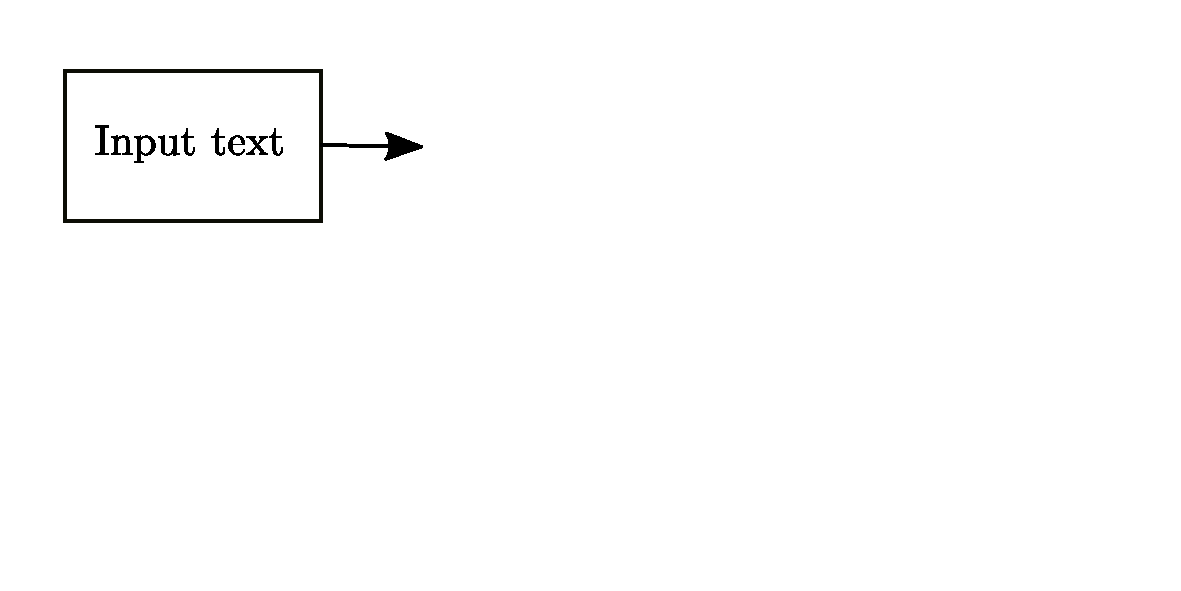
\includegraphics[scale=0.85]{NLP_pipeline}		
		%\captionsetup{justification=centering}
		\caption{The NLP pipeline}
		\label{NLP_pipeline_label}
	\end{figure}
	Let us just address briefly some possible points in the figure. Since sentence splitting produces sentences from an input text, the three arrows represent multiple sentences going into the tokenization block. As already said, it is important to know the sentence boundaries when computing the co-occurrence matrix.
	
	The tokenization block takes as an input the MWE block since it uses the MWE lexicon and other MWE specific features that we mentioned (e.g. abbreviations after the MWE) to correctly tokenize the input.
	
	The lemmatization block which takes in two inputs, the flow of tokens from the previous block and, to function properly, it also needs the PoS tags from the token removal block.
	
	The last point to mention is that after the normalization block, the output is not a single stream of tokens, but rather a list of lists of tokens, where each list represents one sentence that the sentence splitting block separated.
	This figure will be expanded once we talk about other steps required to build the whole model. 

	
	\newpage 
	\section{Word Embeddings}
	\subsection{How to Represent Words as Numbers?}
	The big challenge of any text processing on a computer is how to represent words as numbers? This is a fundamental question in NLP as computers inherently work with numbers and NLP works with words. In contrast to other areas of computer science like image processing and audio processing whose working medium (images and waveforms) can be and are represented with numbers, there is no apparent way on how to represent the working medium of NLP (words) as numbers.
	
	The naive approach would be to map each word in a language to a single number, but, for example, the word "banana" being number $134$ and the word "orange" being number $54$ doesn't tell us anything about those words or the relation between them. A single number cannot meaningfully represent the essence of a word among thousands of other words. The idea is to somehow represent the features of words. For example, the features of "orange" are that it is a fruit, round, orange colored, etc. In contrast, a "banana" is also a fruit but it is curved and yellow. So in that sense, we could encode the features of words as numbers, and measure, for instance, how much is an object round or yellow and so on. The next natural step is to encode those word features as \textit{feature vectors} and this is the point where we come to word embeddings.
	
	\textbf{Word embeddings} are representations of words as real-valued dense vectors such that words which are closer in such a vector space tend to have a similar meaning \cite{word-embedding-survey}. Word embeddings have revolutionized the field of NLP by enabling computers to interpret and understand words. Each entry of the embedding represents a feature of the word. These vectors are in high-dimension spaces as there are tens and even hundreds of features that words have, and they become abstract so that there is no sense in even interpreting them. The higher dimension the better representation of words we have, but there is the computational trade-off, as longer vectors required more resources to process and store. Let us look at an example of a $2$D subspace of a larger, high-dimensional space. We can see how words in such a space are behaving in terms of their embeddings in Figure \ref{subspace_label}.
	\begin{figure}[H]
		\centering
		\hspace*{-1.0cm}
		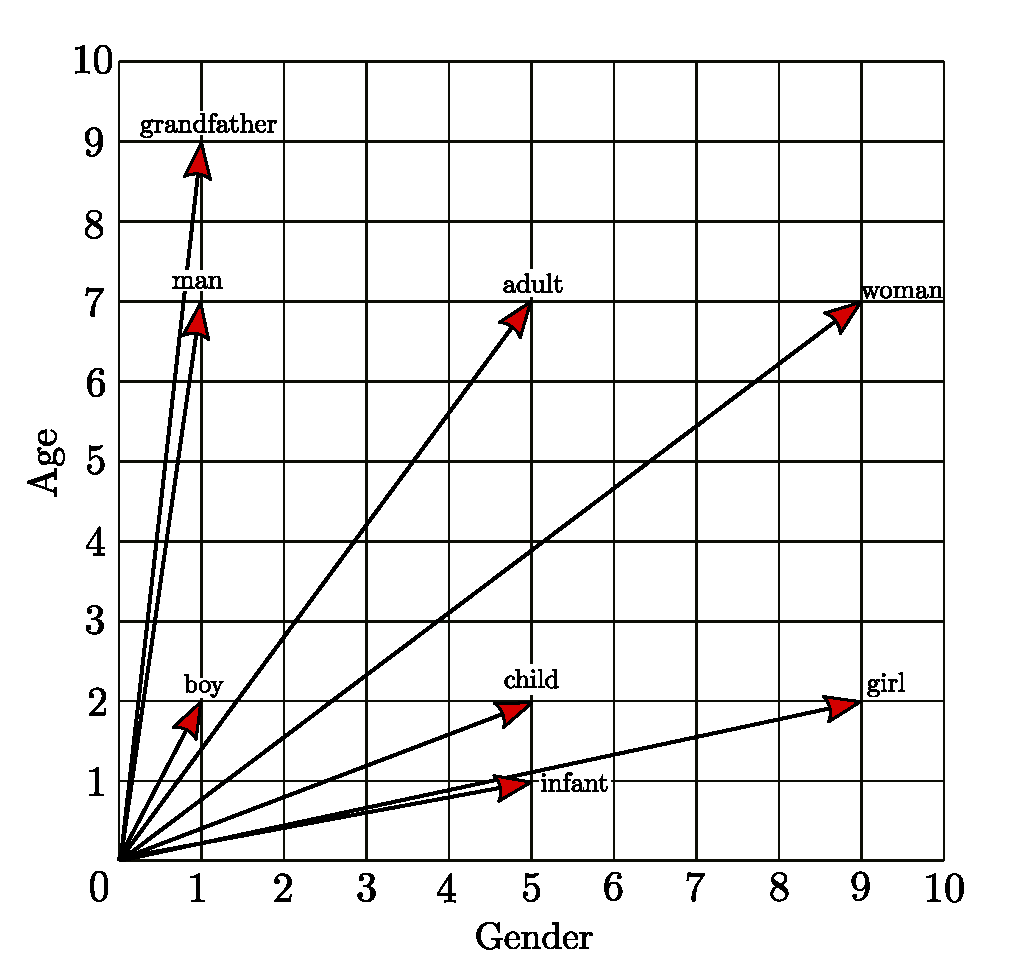
\includegraphics[scale=0.75]{subspace}		
		%\captionsetup{justification=centering}
		\caption{Word embeddings in the Gender-Age subspace}
		\label{subspace_label}
	\end{figure}
	
	The numbers on the Gender and Age axes are just for presentation purpose as word embeddings are usually real-valued which means they are also continuous. The reason for such a representation instead of an integer or one-hot representation is that continuous and dense vectors capture more accurate and subtle semantic relations between words. The other reason is that real-valued embeddings are more efficient for computation than other sparse representations. The vector elements are also usually in the range $[-1, 1]$ for normalization purposes when using them in neural networks. 
	
	As for the example in Figure \ref{subspace_label} we can see that for the Gender axis the lower values are regarded as more male (grandfather, man, boy), the higher values are regarded as more female (woman, girl) and the values in between have no specific gender (adult, child, infant). As for the Age axis, we have the same idea, based on the age of a person the words have higher or lower values. We can see the power of embeddings, as the vector representation of a word does really carry meaning in such a space. And if a new word would be mapped in this space, e.g. "lady" to the vector $(8, 6)$ based on how much the word is "old" or "young" and "male" or "female". We also see that words that are more similar are closer to each other in this space, and they form \textbf{clusters}. This is just a 2$D$ example of a space, but a space with, say $50$ dimensions, will have many more refined features and we can form more refined clusters (e.g. cluster of fruits which are yellow). In Figure \ref{cluster} we can see an example of different word clusters gotten from the "\textit{glove-wiki-gigaword-50}" word embedding model vectors \cite{glove}. One of the ways of obtaining these clusters is using the K-means clustering algorithm (in fact, it is the perfect example of using K-means). 
	\begin{figure}[H]
		\centering

		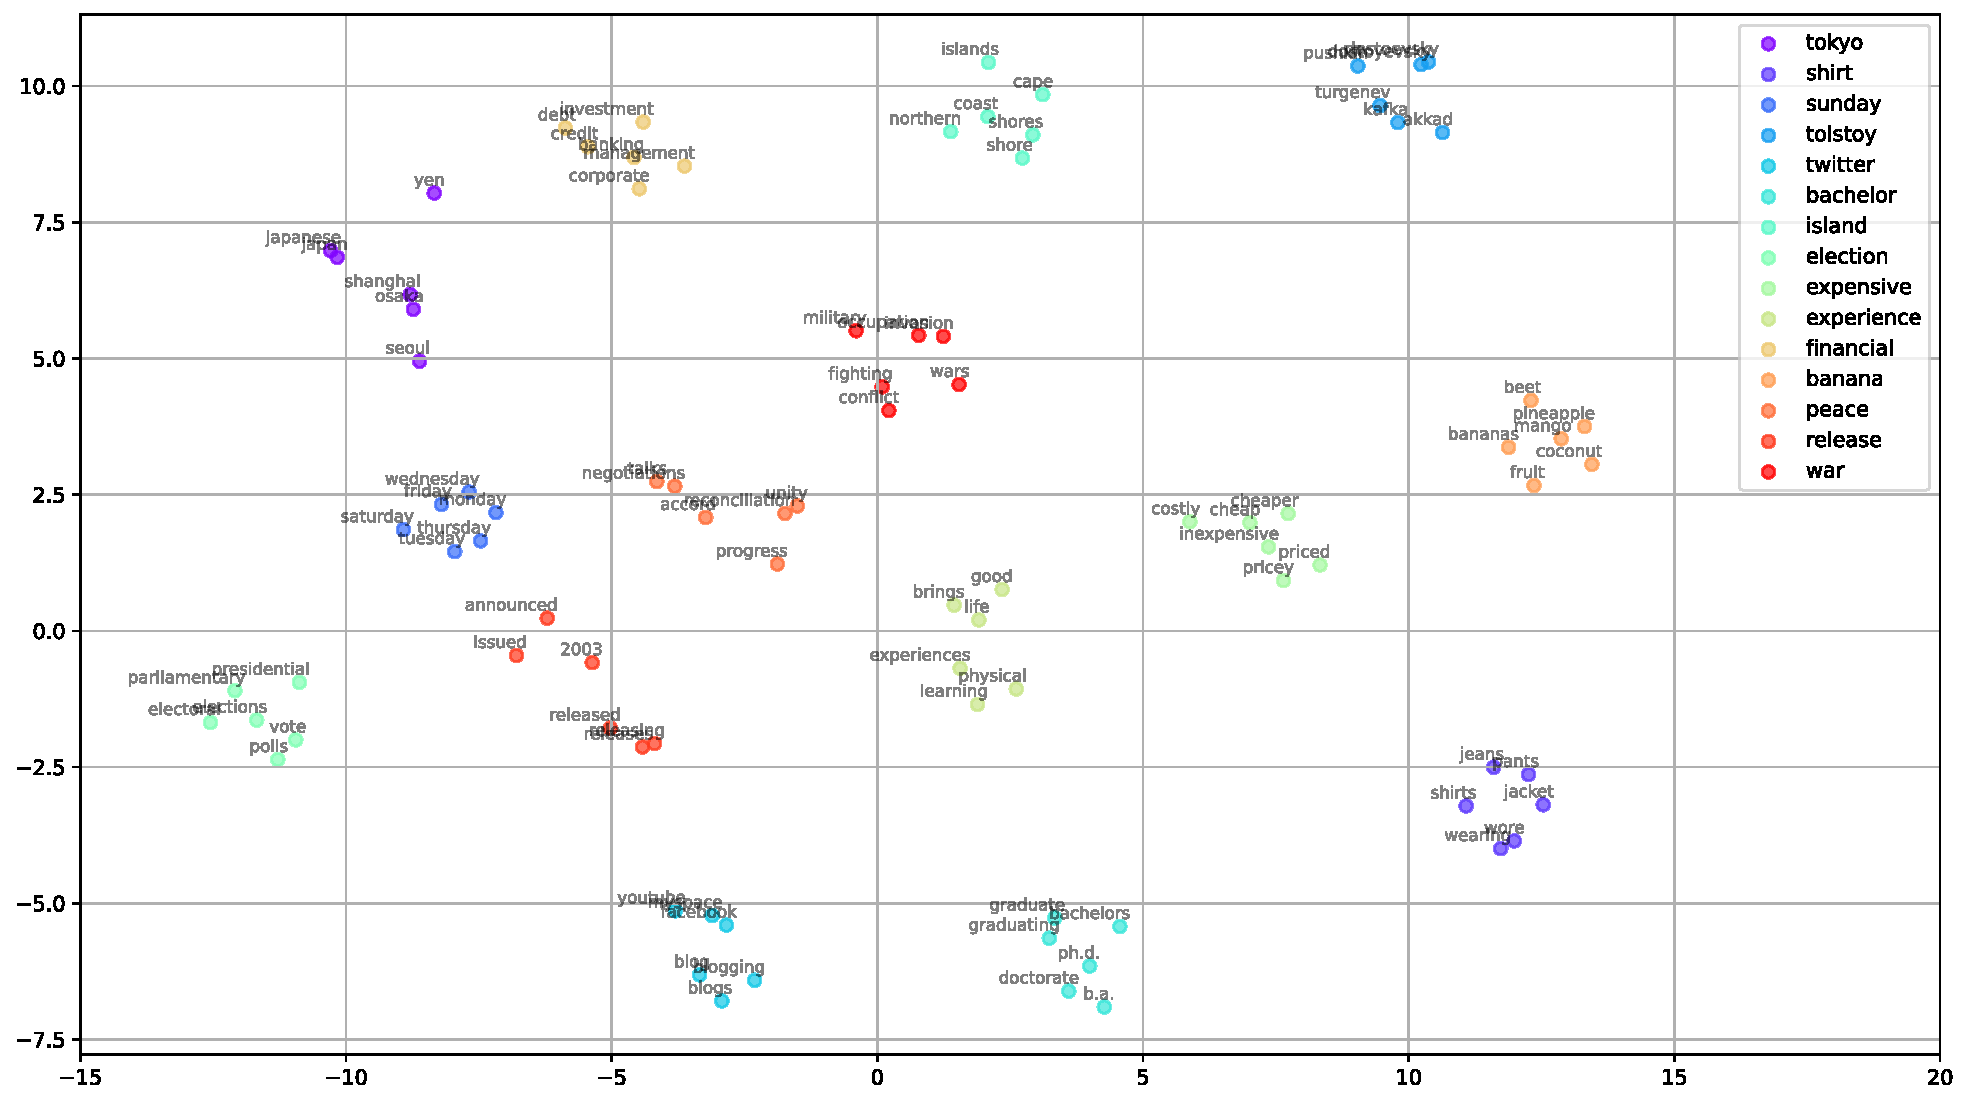
\includegraphics[scale=0.50]{clusters}		
		%\captionsetup{justification=centering}
		\caption{Clusters of words using word embeddings}
		\label{cluster}
	\end{figure}
% https://towardsdatascience.com/google-news-and-leo-tolstoy-visualizing-word2vec-word-embeddings-with-t-sne-11558d8bd4d
	
	The real power of these vectors is that we can perform standard vector operations on them, like the addition and the cosine similarity. This enables us to numerically measure the similarity between words with the cosine similarity like:
	\begin{equation}\label{cosine_similarity}
		S_C(A, B) = \frac{\mathbf{A}\cdot \mathbf{B}}{\|\mathbf{A}\| \| \mathbf{B}\|}
	\end{equation}

	We can test this on the figure with the similarity between "grandfather" and "man" versus "grandfather" and "girl":
	
	$$ S_C(\text{grandfather}, \text{man}) = \frac{(1, 9) \cdot (1, 2)}{\|(1, 9)\| \|(1, 2)\|} = 0.94 $$ 
	$$ S_C(\text{grandfather}, \text{girl}) = \frac{(1, 9) \cdot (9, 2)}{\|(1, 9)\| \|(9, 2)\|} = 0.32 $$ 
	
	We observe the expected, that "grandfather" and "man" are more similar (both male and older) than "grandfather" and "girl" (different genders and ages). The other operation we mentioned was vector addition. Adding and subtracting word embeddings means that we basically add and subtract the features associated with words. Let us show that on an example (where WE means the word embedding of a word):
	$$ \text{WE}(\text{woman}) - \text{WE}(\text{man}) + \text{WE}(\text{boy}) = (9, 7) - (1,7) + (1, 2) = (9, 2) = \text{WE}(\text{girl})$$
	
	The intuition behind the addition and subtraction for this example is that we subtracted the age from "woman" with the age of "man" (which gives $0$ age), and gender from "boy" with the gender of "man" (which gives $0$ gender) and added the age from "boy" and gender from "woman" which gives us something that has the age of a boy and the gender of a woman. That something is a girl, which is exactly what we got. Doing this in higher dimensions we can get the closest cluster to the resulting vector and get a set of words which are similar to the desired output.
	
	\subsection{How are Word Embeddings Computed?}
	We have seen what word embeddings are, their functionalities and how to use them, but how do we actually compute them, in an automated way? \\
	
	To core concept of obtaining word embeddings is that similar words occur in the same context. This means that words that are close together in a text also tend to be similar to each other. This is also known as the \textbf{distributional hypothesis} \cite{distributional}. This is a strong hypothesis but it has been proven to be viable. The most successful models for calculating word embeddings are neural network based using the context assumption. The neural networks are usually shallow as the network weights are used as the embeddings \cite{word-embedding-survey}. The idea is to use a \textbf{skip-gram} model, which takes a target word and tries to predict the surrounding context words. A sliding window is used for the size of the context. Then the target word is used as the input to the neural network (actually the one hot encoded sliding window) and the preceding and succeeding words in the context are predicted as the output (which we know). The network is then trained to minimize the difference between the predicted word and actual word in the context. The network weights are adjusted during the training to improve the accuracy of the predictions using the backpropagation algorithm. The resulting weights of the hidden layer are used as the word embeddings as they capture the semantic relationships between words \cite{word-embedding-survey}. This skip-gram architecture is used in Google's \textbf{word2vec} word embeddings toolkit \cite{word2vec} developed in $2013$.
	% https://medium.com/@corymaklin/word2vec-skip-gram-904775613b4c
	% https://www.turing.com/kb/guide-on-word-embeddings-in-nlp
	
	The other way of getting the embeddings is using global statistical information of the entire corpus constructing a co-occurrence matrix. That matrix represents the frequency of word pairs occurring together in a given context window. This is exactly the way we will get the pair-wise connections of nodes in the graph we will build. The obtained matrix is then factorized to the final embeddings (the process has some more details but we won't go into detail). This co-occurrence matrix architecture is used in the \textbf{GloVe} model \cite{glove}.
	
	When the word embeddings are obtained, they are usually saved in a data object similar to a dictionary where the key is the word and the value is the word embedding. This is an efficient way of getting the embedding values for a specified word. One can train their own model on their own data, but there are many pre-trained models, and the embeddings can be used directly.
	
	Some apparent problems using word embeddings as they were described are:
	\begin{enumerate}
		\item How to embed phrases (or MWE)?\\
		When training the network on target words, we can define \textit{target phrases} instead of words. A model called phrase2vec \cite{phrase2vec} exclusively built for phrase embedding. There are also models which can embed sentences as vectors, so we can treat sentences as phrases.
		\item How to deal with homonymy (words with different meaning but written the same)? \\
		To overcome this problem, \textit{multi-sense} embeddings can be used, where a word can be mapped to more embeddings considering a word's context \cite{multi_sense_we}. 
	\end{enumerate}
	
	Once the graph is built, with words as nodes and the edges as connections between the words gotten from the co-occurrence matrix, we can alter the weights of the edges by multiplying them with the cosine similarity of the embeddings between two adjacent nodes. In this way we aim to strengthen (or loosen) the semantic link between words.
	
	
	\newpage
	\section{Graph Construction}
	In this section we will dive into the construction of the graph model. A graph $\mathcal{G}$ is defined as an ordered pair:
	\begin{equation}
		\mathcal{G} = (\mathcal{V},\mathcal{E})
	\end{equation}
	where $\mathcal{V}$ is the set of nodes and $\mathcal{E}$ is the set of edges, the links between adjacent nodes \cite{juricGrafovi}. We will model the text to be analyzed as a graph. The set of nodes are going to be the tokenized words. The more important question is what are going to be the edges?
	Well, we need to somehow encode the links (semantic relation) between words. We are going to use the same hypothesis word embeddings use, that words that occur in similar contexts tend to have similar meanings. If words occur in the same context, we will link them with an edge, and in such a way we will encode the links between words. An important note is that the graph is going to be \textit{undirected} which means that the edges are bidirectional i.e. they don't have an orientation. In this way we are not preserving the word order, as we will not need it, but for some other tasks it could be useful to have it.
	
	There are different data structure representations of graphs, e.g. as an \textit{adjacency list}, \textit{adjacency matrix}, etc. In the Figure \ref{graph_adjacency} we can see a graphical and matrix representation of a weighted graph. Each entry in the matrix corresponds to an edge between two nodes and its respective weight (weight of $0$ means the nodes are not connected).
	
	\begin{figure}[H]
		\centering
		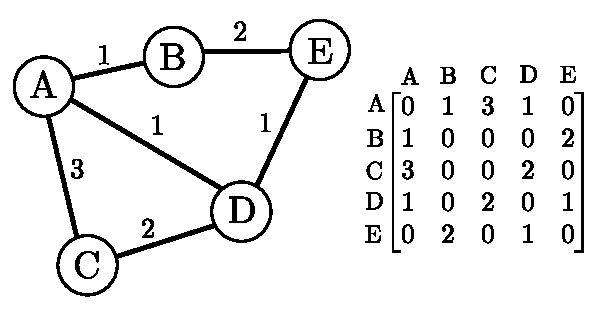
\includegraphics[scale=1.0]{graph_adjacency}		
		%\captionsetup{justification=centering}
		\caption{Example of weighted graph and its adjacency matrix}
		\label{graph_adjacency}
	\end{figure}

	We are going to use an adjacency matrix representation for visualization purposes as it is a good way to translate between graphs and text but in the actual implementation we will use an adjacency list as adjacency matrices are usually sparse. This is especially true as we will express the \textit{distributional hypothesis} as a co-occurrence matrix which we will explain in the next subsection. 
	
	\subsection{Co-occurrence matrix}
	% https://www.baeldung.com/cs/co-occurrence-matrices
	A \textbf{co-occurrence matrix} in NLP is a matrix that represents the frequency of word co-occurrences within a specified context window for a given text. The idea is to capture how often words appear together in similar contexts. For a given context window size we see how many pair-wise combinations there are. Each row and column of the matrix corresponds to a unique word in the vocabulary \footnote{Set of unique words in a corpus also knows as \textit{types}} and the matrix elements contain the count of pair-wise word occurrences. 
	
	We will respect sentence boundaries, so that the context window cannot be present across two or more sentences but just one. The reason is that adjacent sentences might not refer to the same context so we will analyze them independently. In Figure \ref{NLP_pipeline_label} the output text is assumed to be a set of tokenized sentences, which means that for each sentence after the sentence splitting module we perform all the steps and get all the tokens per sentence.
	
	Let us look at an example set of sentences, for which we are going to perform the NLP pipeline, perform the context window sliding with a window size of $3$ words and show the co-occurrence matrix.
	
	We can see in the diagram \ref{co_matrix_construction} that we have an input of three sentences which go through the NLP pipeline and we obtain the tokenized sentences (which went also through all the other steps of the NLP pipeline). The next step is the co-occurrence calculation. The sliding window is visualized as the context words are marked red and the window is sliding until it reaches the end of the sentence after which it goes to the next sentence. The last step is the aggregation of the number of pair-wise co-occurrences into the co-occurrence matrix.
	
	
	\begin{figure}[H]
		\vspace{-0.5cm}
		\centering
		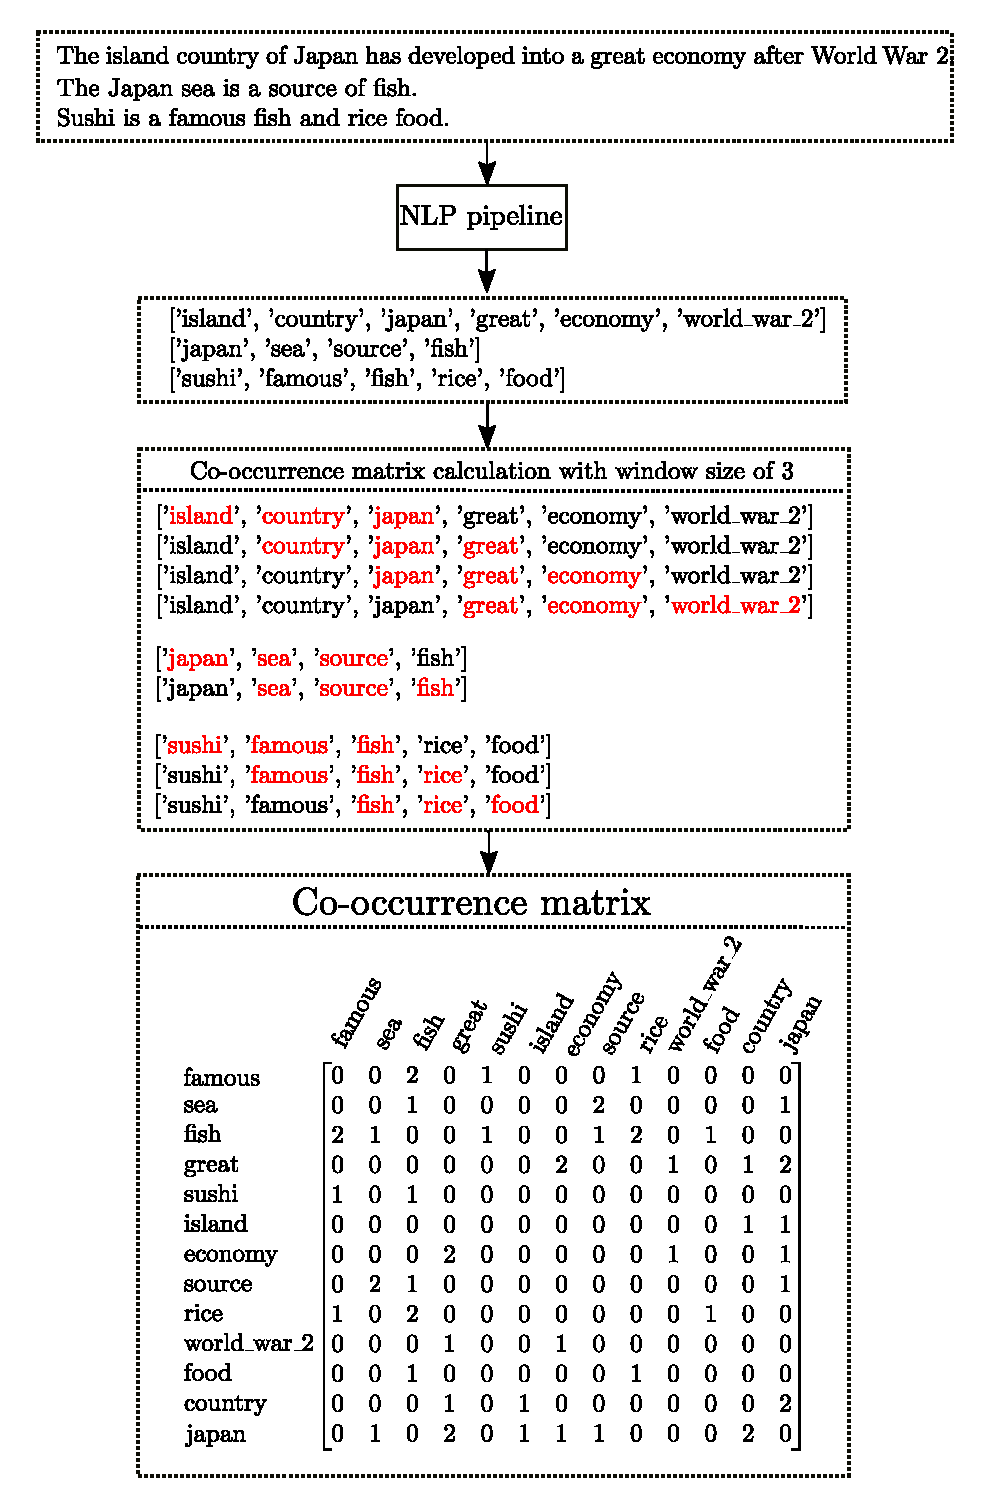
\includegraphics[scale=0.85]{context_diagram}		
		%\captionsetup{justification=centering}
		\caption{Co-occurrence matrix construction}
		\label{co_matrix_construction}
	\end{figure}
	
	The co-occurrence matrix is in a one-to-one relationship to a graph's adjacency matrix so we can get a graph representation directly from the co-occurrence matrix. One thing to note is that the co-occurrence matrix in the Figure \ref{co_matrix_construction} is sparse, so for memory purposes, we actually store the adjacency matrix as a dictionary (a version of the adjacency list) where the keys are the pair-wise word occurrences and the values are the number of co-occurrences (the graph weights).
	In Figure \ref{graph_example} we can see the graph representation of the example above.
	
	\begin{figure}[H]
		\centering
		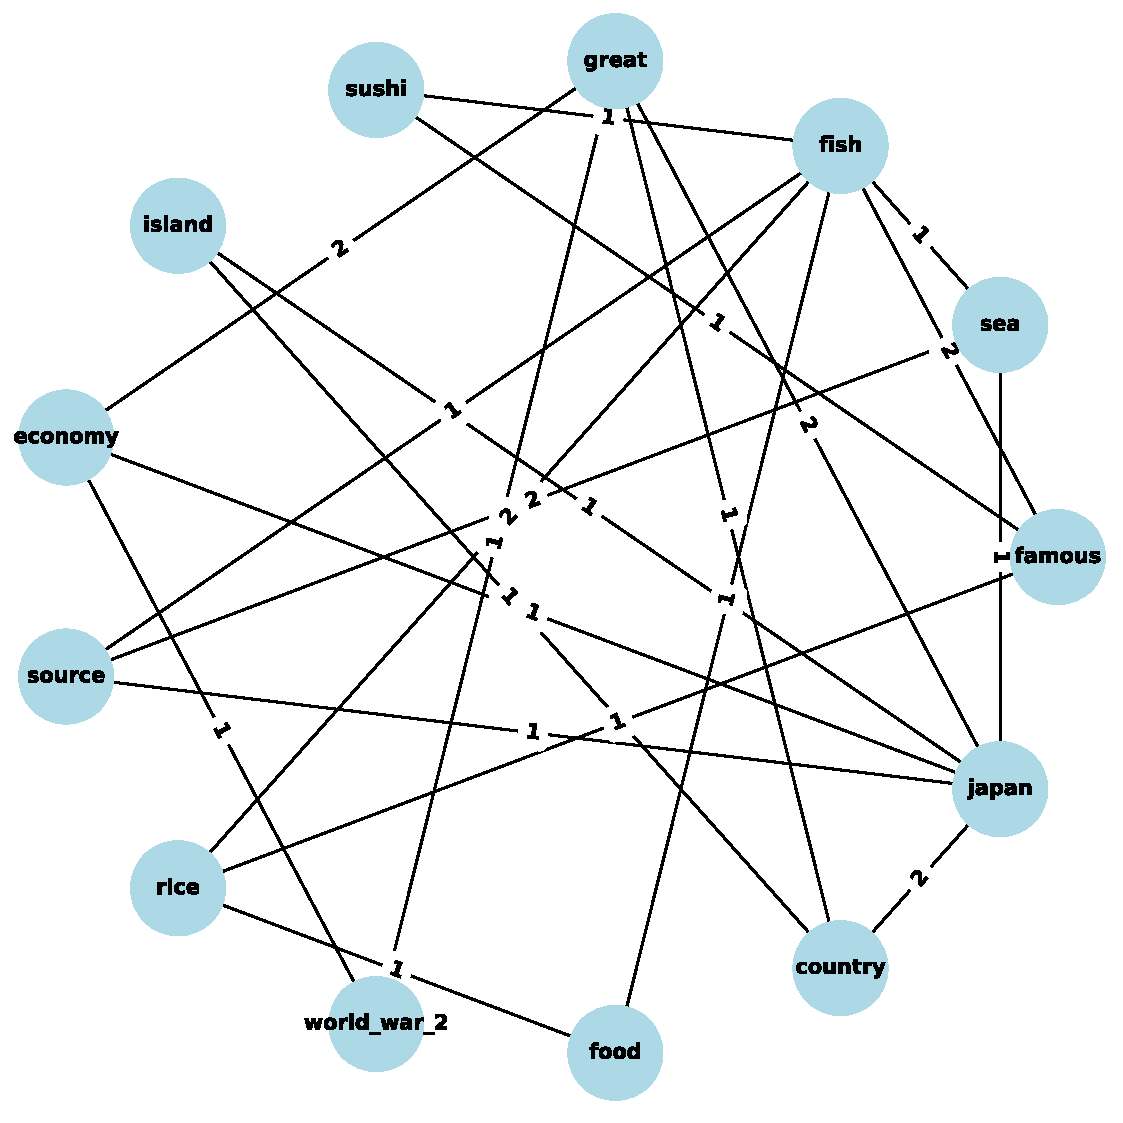
\includegraphics[scale=0.80]{graph_example}		
		%\captionsetup{justification=centering}
		\caption{Graph representation of the co-occurrence matrix}
		\label{graph_example}
	\end{figure}

	Just by looking at the graph we can observe that "japan" has the most edge connections. We can also see the semantic relationship between words and their respective strength like (japan, country, $2$), (sushi, fish, $1$), (rice, food, $1$), etc.
	
	The last step in the graph construction is to encode the word-embedding values in the graph. It is enough to find the cosine-similarity between adjacent nodes and multiply the edge weight with the value of the similarity between words.
	We can now visualize the whole keyword extraction pipeline in Figure \ref{full_pipeline}.
	
	\begin{figure}[H]
		\centering
		\hspace*{-1cm}
		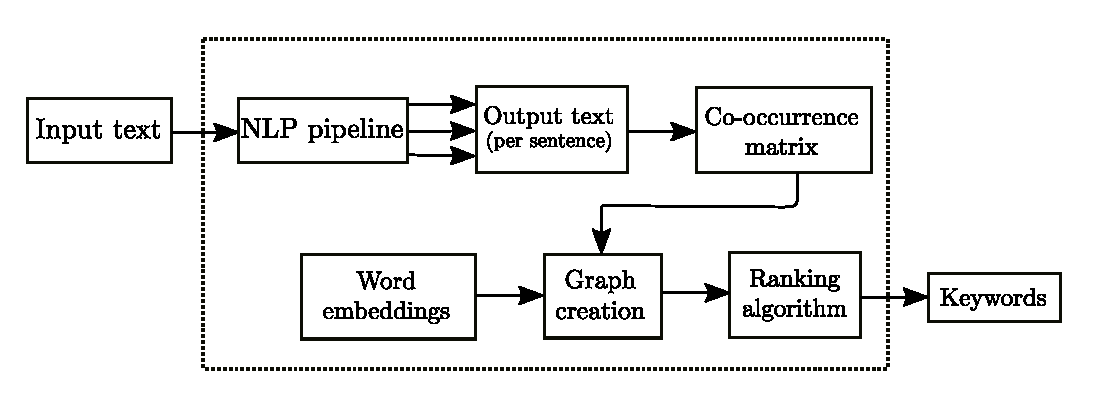
\includegraphics[scale=1.0]{full_pipeline}		
		%\captionsetup{justification=centering}
		\caption{Full pipeline of keyword extraction}
		\label{full_pipeline}
	\end{figure}
	
%	We can see that the last block before obtaining the keywords is the \textit{ranking algorithm}. In the next chapter we will discuss how to rank nodes in a graph based on different graph features, whose output are going to be the keywords.
	
	\newpage
	\section{Implementation of Keyword Extraction from Graphs}
	The last, and frankly, most important step is the actual ranking of the words in the graph. Based on this ranking we will get the most important nodes. There are many different ranking algorithms to rank graph nodes, which take into account node connections, edge number, edge weights, etc. 
	
	\subsection{Degree centrality}
	Degree centrality is a measure that quantifies the importance of nodes in a graph based on the number of edges connected to them \cite{networkx_centrality}. The number of edges connected to a node in a graph is called it's \textit{degree}. The degree of a node can also be thought of as the number of non-zero values in the row or column of the given node in the adjacency matrix. The formula for degree centrality is given as:
	\begin{equation}
		C_d(v) = \frac{\deg(v)}{|\mathcal{V}|-1}
	\end{equation}
	We divide the node degree by the number of nodes minus $1$ to normalize the degree centrality, so that all the values are in the range $[0, 1]$. In the Figure \ref{graph_example} we can check the degree centralities of a few different nodes like 
	$$C_d(\text{japan}) = \frac{\deg\text{(japan)}}{|\mathcal{V}|-1} = \frac{6}{13-1} = 0.50$$
	$$C_d(\text{sea}) = \frac{\deg\text{(sea)}}{|\mathcal{V}|-1} = \frac{3}{13-1} = 0.25$$
	We can see that the edge weights are not considered in this ranking algorithm. From the standpoint of text, words with high degree centrality would be the ones which are frequently present in the context windows of other words. However this might not capture the full semantic meaning as we are not looking at the weights of the edges. Nevertheless, this algorithm gives us still a simple but effective way to rank words in a text. 	
	
	\subsection{Closeness centrality}
	Closeness centrality is a measure that quantifies how close a node is to other nodes in a graph \cite{bavelas}. This notion of closeness is the defined as the inverse of the sum of the shortest distances from a node to all the other nodes in the graph. It usually contains the factor of $|\mathcal{V}|-1$ to normalize the formula, so it has the following form:
	\begin{equation}
		C_c(v) = \frac{|\mathcal{V}|-1}{\sum_{u=1}^{|\mathcal{V}|} d(u,v)}
	\end{equation}
	where $d(u,v)$ is the shortest distance between nodes $u$ and $v$. When talking about the distance between two adjacent nodes, that distance is the edge weight. So, the shortest distance between any two nodes is the set of edges which connect the two nodes such that the sum of their weights is minimal. The most famous algorithm used for finding the shortest distance between two nodes in a graph is Dijkstra's algorithm \cite{dijkstra}. In the case that the graph in not completely connected, the closeness centrality would be computed for each connected part separately and then scaled by the size of that part. 
	
	In Figure \ref{graph_adjacency} the shortest distance between nodes $A$ and $E$ is $2$ along the path $A - D - E$ even though from the figure it might look like it is the path $A - B - E$ but that path has a distance of $3$. We can calculate the closeness centrality for "japan" in Figure \ref{graph_example}: 
	\begin{equation*}
		\begin{split}
			C_c(\text{japan}) & = \frac{|\mathcal{V}|-1}{d(\text{source},\text{japan}) + \cdots + d(\text{sushi},\text{japan}) + \cdots + d(\text{world\_war\_2},\text{japan})} \\
			& = \frac{12}{|\text{source, japan}| + \cdots |\text{sush, fish, sea,  japan}| + \cdots + |\text{world\_war\_2, economy, japan}|} \\
			& = \frac{12}{1 + \cdots + 3 + \cdots + 2} \\
			& = \frac{12}{26}
		\end{split}
	\end{equation*}
	In this manner the closeness can be calculated for all the other nodes. The meaning of the obtained closeness score is that higher scores are assigned to nodes that are, on average, closer to all the other nodes in the graph. An intuitive example is when cities and the roads between them are modeled as graphs. Then, the cities which are well connected to other cities and located centrally in a country have higher closeness scores (e.g. Madrid vs. Barcelona in Spain).  
	
	When it comes to text, words with high closeness scores are on average closer to other words which means that they are central to the concept and the overall flow of information in text. Such words are potentially important for understanding the core meaning or theme of the text, as they are well-connected to other words and might play a crucial role in conveying the context. They could also act as bridges between different parts of the text (e.g. in example Figure \ref{co_matrix_construction}, Japan connects the first two sentences and fish connects the second and third sentence).
	
	\subsection{Betweenness centrality}
	Betweenness centrality is a measure of node's centrality based on its part in facilitating the flow of information between other nodes. The flow of information in a graph is governed by the shortest paths between respective nodes. The betweenness centrality for each node is the number of these shortest paths that pass through that node. This is defined mathematically as:
	\begin{equation}
		C_B(v) = \sum_{s,t \in \mathcal{V}} \frac{\sigma(s, t|v)}{\sigma(s,t)}
	\end{equation}
	where $\sigma(s,t)$ is the number of shortest paths between nodes $s$ and $t$, and $\sigma(s, t|v)$ is the number of those paths that pass through node $v$. If $v \in \{s, t\}$ then $\sigma(s, t|v) = 0$ \cite{freeman}. This expression is usually normalized by multiplying it by the factor $\frac{2}{(|\mathcal{V}| -1)(|\mathcal{V}| - 2)}$. One thing to note is that, the shortest path between two nodes is not unique, there might be more than one path that has the minimum distance between two nodes (e.g. in Figure \ref{graph_adjacency} the distances of paths $A - C$ and $A - D - C$ between nodes $A$ and $C$ are the same).
	
	Betweenness centrality quantifies the number of times a node serves as a bridge along the shortest paths between pairs of other nodes in the graph. Nodes with high betweenness centrality play a crucial role in maintaining efficient flow and connectivity within a graph. Calculating the betweenness score can be quite tiresome when doing it by hand for larger graphs, so instead of the example in Figure \ref{graph_example} we will show how the example in Figure \ref{graph_adjacency}. Let us firstly list all the pairs of nodes that have more than one shortest path:
	\begin{flushleft}
		$A$ to $C$: $A - C$, $A - D - C$ \\
		$A$ to $E$: $A - D - E$ \\
		$B$ to $C$: $B - A - C$, $B - A - D - C$ \\
		$B$ to $D$: $B - A - D$ \\
		$C$ to $E$: $C - D - E$ \\
	\end{flushleft}
	We see that only nodes $A$ and $D$ appear as a part of the shortest paths so all the other nodes have $0$ betweenness centrality. Let us see the scores for the nodes $A$ and $D$:
	\begin{equation*}
		\begin{split}
			C_B(A) & = \sum_{s,t \in \mathcal{V}} \frac{\sigma(s, t|A)}{\sigma(s,t)} = \frac{\sigma(A, C|A)}{\sigma(A, C)} + \frac{\sigma(A, E|A)}{\sigma(A, E)} + \frac{\sigma(B, C|A)}{\sigma(B, C)} + \frac{\sigma(B, D|A)}{\sigma(B, D)} + \frac{\sigma(C, E|A)}{\sigma(C, E)} \\
			& = \frac{0}{2} + \frac{0}{1} + \frac{2}{2} + \frac{1}{1} + \frac{0}{1} = 2 \\
			C_B(D) & = \sum_{s,t \in \mathcal{V}} \frac{\sigma(s, t|D)}{\sigma(s,t)} = \frac{\sigma(A, C|D)}{\sigma(A, C)} + \frac{\sigma(A, E|D)}{\sigma(A, E)} + \frac{\sigma(B, C|D)}{\sigma(B, C)} + \frac{\sigma(B, D|D)}{\sigma(B, D)} + \frac{\sigma(C, E|D)}{\sigma(C, E)} \\
			& = \frac{1}{2} + \frac{1}{1} + \frac{1}{2} + \frac{0}{1} + \frac{1}{1} = 3
		\end{split}
	\end{equation*}
	And normalizing the results we get $C_B(A) = 1/3$ and $C_B(D) = 1/2$.
	
	When it comes to text, words with high betweenness scores act as "bridges" or "connectors" between different parts of text, as they might appear in position which link distinct text concepts. On the other hand, words with low scores may be isolated or play a more local role on a sentence or phrase level rather than a text level.
	
	\subsection{Eigenvector centrality}
	Eigenvector centrality is a measure of the importance of a node in a graph, taking into account both its direct connections to other nodes, and the connections of its neighbors \cite{networkx_centrality}. A node has a high eigenvector centrality score if it is connected to other nodes that have a high score. The eigenvector score of node \textit{i} is defined as the sum of the scores of its neighbors multiplied by the edge weights and scaled by a factor $\lambda$. Let $\mathbf{A}$ be the adjacency matrix of a graph $\mathcal{G}$, where the entry $a_{v,t}$ of $\mathbf{A}$ is the edge weight between nodes $v$ and $t$ then the centrality score $x_v$ of node $v$ is defined as:
	\begin{equation}\label{eigenvector_1}
		x_v = \frac{1}{\lambda} \sum_{t \in \mathcal{V}} a_{v,t} x_t
	\end{equation}
	doing this for all the nodes in the graph, the equation can be rewritten in matrix notation as:
	\begin{equation}\label{eigenvector_2}
		\mathbf{A}\mathbf{x} = \lambda \mathbf{x}
	\end{equation}
	which is the definition of an eigenvector, hence the name eigenvector centrality. The scaling factor $\lambda$ is the eigenvalue assigned to the eigenvector. The number of eigenvalues for the adjacency matrix $\mathbf{A}$ is going to be the number of nodes $|\mathcal{V}|$, so which one do we choose?
	
	The centrality score of the \textit{i}-th node is obtained as the \textit{i}-th component of the eigenvector $\mathbf{x}$ with the highest eigenvalue $\lambda$ (also called the \textit{dominant eigenvector}). This condition of using the dominant eigenvector for the scores comes from the fact that the scores have to be positive \cite{networkx_centrality}. \footnote{By the Perron-Frobenius theorem a real square matrix with positive entries has a unique eigenvalue of largest magnitude and the eigenvalue is real. The corresponding eigenvector can be chosen to have strictly positive components.} The eigenvector is defined up to the eigenvalue $\lambda$, so only the ratios of the centralities of the nodes are well defined. We can go a step further to make sure that the scores are in the range $[0, 1]$ by using the unit vector $\mathbf{x}/||\mathbf{x}||$. Let us demonstrate this ranking algorithm on the graph in Figure \ref{graph_adjacency} where we get that the dominant eigenvector is:
	$$ \mathbf{x} = 
	\begin{bmatrix}
		2.738 & 1.087 & 2.887 & 2.183 & 1
	\end{bmatrix}^{T}, \text{with eigenvalue of } \lambda = 4.358$$
	and scaling $\mathbf{x}$ with $||\mathbf{x}||$ we get the scores as:
	$$ \frac{\mathbf{x}}{||\mathbf{x}||} = \begin{bmatrix}
		0.574 & 0.228 & 0.605 & 0.457 & 0.209
	\end{bmatrix}^{T}$$ 
	We can check if the scores of the neighboring nodes add up as stated in equation \ref{eigenvector_1} for the node $C$ as:
	$$ x_C = \frac{1}{\lambda} (a_{C,A}x_A + a_{C, D}x_D) = \frac{3 \cdot 0.574 + 2 \cdot 0.457}{4.358} = 0.605 = x_C $$
	From the graph in Figure \ref{graph_adjacency} we can see that even though the node $C$ is not central it has a high score as it is connected to nodes which have a high score and are central. 
	
	The usual way to calculate eigenvalues are using the \textit{characteristic polynomial} as $\det(A-\lambda I) = 0$ but we do not need all the eigenvalues, just the one with the largest magnitude. Taking this into account, in practice when calculating the dominant eigenvector the \textbf{power iteration} algorithm \cite{networkx_centrality} is used. It is an iterative algorithm which returns the eigenvalue $\lambda$ which is the greatest eigenvalue of $A$ in magnitude and the eigenvector $\mathbf{x}$ assigned to it. The iterative recurrence relation is defined as:
	\begin{equation}
		\mathbf{b}_{k+1} = \frac{\mathbf{A}\mathbf{b}_{k}}{|| \mathbf{A}\mathbf{b}_{k}||}
	\end{equation}
	where $\mathbf{b}_{k}$ is the eigenvector in the \textit{k}-th iteration.
	The stopping condition can be defined in various ways such as the maximum number of iterations or a threshold in the change of the eigenvector in consecutive iterations.
	
	When it comes to text, words with high eigenvector scores have either direct connections to important words or are themselves important words. On the other hand, low scores indicate that the words are less central to the main topic of the text and that they are more local to specific sentences.
	
	\subsection{PageRank (TextRank) algorithm}
	PageRank is a ranking algorithm, originally used by Google's search engine to rank web pages in the search engine results \cite{pagerank}. The internet can be modeled as a graph where the web pages are the nodes and the hyperlinks between them are the edges. This idea can be applied to text as well, where the variation of the algorithm is called \textbf{textrank} \cite{textrank} but we will keep the name PageRank as the ranking algorithm.
	
	The basic idea behind the algorithm is the notion of \textit{casting votes}. When one node links to another is casts a vote for the that other node. The higher the number of votes for a node, the higher the importance for that node. The importance of the vote that was casted by the initial node is influenced by the importance of that node itself. For a weighted graph, the vote of node $j$ to node $i$ is scaled by the ratio of the $(i,j)$ edge weight to the sum of all the edge weights of node $j$. In this way only a part of the $j$ node's vote is casted towards node $i$. Casting all the votes towards the node $i$ we get the following recurrence relation for the PageRank (PR) score: 
	\begin{equation}\label{pagerank1}
		PR(v_i) = \sum_{v_j \in N(v_i)} \frac{w_{j,i}}{\sum_{v_k \in N(v_j)} w_{j,k}} PR(v_j) 
	\end{equation}
	where $N(v_i)$ is the set of all the neighbors of node $i$ and $w_{i,j}$ is the edge weight between nodes $i$ and $j$. The mentioned weight ratio can be obtained from the adjacency matrix if the matrix is converted to a \textit{left stochastic matrix} \footnote{A left stochastic matrix is a square matrix, with each column summing to 1.} One thing to note is that the maximum magnitude of the eigenvalue of a stochastic matrix is $1$ to which the dominant eigenvector is associated.
	
	Let us call the left stochastic matrix of the adjacency matrix $\mathbf{P}_\mathbf{A}$ and the vector containing the PageRank values for all the nodes $\mathbf{R}$, then the equation \ref{pagerank1} can be rewritten in matrix notation as:
	\begin{equation}\label{pagerank2}
		\mathbf{R} = \mathbf{P}_\mathbf{A} \mathbf{R}
	\end{equation}
	which is the same form as the equation \ref{eigenvector_2} where $\lambda = 1$ for \ref{pagerank2} as already said. So, the PageRank algorithm is reduced to the eigenvector centrality. The eigenvector $\mathbf{R}$ is also called the \textit{stationary probability vector} as its values (scores) sum to $1$ and the stationary part means that the vector does not change under the application of the $\mathbf{P}_\mathbf{A}$ matrix. 
	
	Let us show the PageRank algorithm on the example from Figure \ref{graph_adjacency} by getting the left stochastic matrix first:
	$$
	\mathbf{A} = 
	\renewcommand\arraystretch{0.8} 
	\begin{bmatrix}
			0 & 1 & 3 & 1 & 0 \\
			1 & 0 & 0 & 0 & 2 \\
			3 & 0 & 0 & 2 & 0 \\
			1 & 0 & 2 & 0 & 1 \\
			0 & 2 & 0 & 1 & 0
		\end{bmatrix},
	\mathbf{P}_\mathbf{A} = 
	\renewcommand\arraystretch{0.8} 
	\begin{bmatrix}
		0 & 0.33 & 0.6 & 0.25 & 0 \\
		0.2 & 0 & 0 & 0 & 0.67 \\
		0.6 & 0 & 0 & 0.5 & 0 \\
		0.2 & 0 & 0.4 & 0 & 0.33 \\
		0 & 0.67 & 0 & 0.25 & 0
	\end{bmatrix}
	$$
	The dominant eigenvector after normalization has the following value: 
	$$ \mathbf{R} = \begin{bmatrix}
		0.25 & 0.15 & 0.25 & 0.20 & 0.15
	\end{bmatrix}^T, \text{with eigenvalue of } \lambda = 1 $$
	Let us confirm this result by calculating the $PR$ score from equation \ref{pagerank1} for the node $A$:
	\begin{equation*}
		\begin{split}
			PR(A) & = \sum_{v_j \in \{B, C, D\}} \frac{w_{j, A}}{\sum_{v_k \in N(v_j)} w_{j,k}} PR(v_j) \\
			& = \frac{w_{B,A}}{w_{B,A} + w_{B,E}} PR(B) + \frac{w_{C,A}}{w_{C, A} + w_{C, D}} PR(C) + \frac{w_{D,A}}{w_{D,A} + w_{D, C} + w_{D, E}} PR(D) \\
			& = \frac{1}{1 + 2}0.15 + \frac{3}{3 + 2}0.25 + \frac{1}{1 + 2 + 1}0.20 \\
			& = 0.25 = PR(A)
		\end{split}
	\end{equation*}
	When it comes to text, words with high PageRank scores are central concepts and they are likely to be connected to other important words in the text (the same concept as web pages and web search) \cite{textrank}. 
	
%	\subsection{Katz centrality}
%	Katz centrality is a measure of node centrality in a graph, which takes into account both the number of neighbors of a node and the centrality of those neighbors. In fact, it is a generalization of the eigenvector centrality with two parameters which influence the value of the centrality score. The mathematical notation of Katz's centrality for a node $x_v$ is defined as:
%	\begin{equation}
%		x_v = \alpha \sum_{t \in \mathcal{V}} a_{v,t} x_t + \beta
%	\end{equation}
%	where the parameter $\alpha$ controls the influence of the influence of the neighboring nodes and it is constrained as $ \alpha \in (0, 1/\lambda_{max}) $ and the parameter $\beta$ controls the initial centrality of the node. The equation can be also written in matrix notation as:
%	\begin{equation}
%		\mathbf{x} = \alpha \mathbf{A}\mathbf{x} + \beta \mathbf{1}
%	\end{equation}
%	The scores $\mathbf{x}$ are also usually scaled to a unit vector. The main 
	
	\subsection{Comparing the ranking algorithms}
	To conclude this section let us apply all the ranking algorithms on the example graph from Figure \ref{graph_example} that models the sentences from Figure \ref{co_matrix_construction} in the form of a table.
	\begin{table}[H]
		\label{table1}
		\centering
		\caption{Ranking values for the example in Figure \ref{graph_example}.}
		\scalebox{0.70}{
		\begin{tabular}{|cc|cc|cc|cc|cc|}
			\hline
			\multicolumn{2}{|c|}{Degree Centrality}      & \multicolumn{2}{c|}{Closeness Centrality}   & \multicolumn{2}{c|}{Betweenness Centrality} & \multicolumn{2}{c|}{Eigenvector Centrality} & \multicolumn{2}{c|}{PageRank}                \\ \hline
			\multicolumn{1}{|c|}{Word}          & Ranking & \multicolumn{1}{c|}{Word}          & Ranking & \multicolumn{1}{c|}{Word}          & Ranking & \multicolumn{1}{c|}{Word}          & Ranking & \multicolumn{1}{c|}{Word}          & Ranking \\ \hline
			\multicolumn{1}{|c|}{japan}         & 0.5     & \multicolumn{1}{c|}{japan}         & 0.462   & \multicolumn{1}{c|}{japan}         & 0.566   & \multicolumn{1}{c|}{japan}         & 0.515   & \multicolumn{1}{c|}{fish}          & 0.148   \\ \hline
			\multicolumn{1}{|c|}{fish}          & 0.5     & \multicolumn{1}{c|}{source}        & 0.444   & \multicolumn{1}{c|}{fish}          & 0.505   & \multicolumn{1}{c|}{great}         & 0.431   & \multicolumn{1}{c|}{japan}         & 0.148   \\ \hline
			\multicolumn{1}{|c|}{great}         & 0.333   & \multicolumn{1}{c|}{sea}           & 0.444   & \multicolumn{1}{c|}{source}        & 0.227   & \multicolumn{1}{c|}{country}       & 0.33    & \multicolumn{1}{c|}{great}         & 0.111   \\ \hline
			\multicolumn{1}{|c|}{country}       & 0.25    & \multicolumn{1}{c|}{fish}          & 0.429   & \multicolumn{1}{c|}{sea}           & 0.227   & \multicolumn{1}{c|}{economy}       & 0.309   & \multicolumn{1}{c|}{famous}        & 0.074   \\ \hline
			\multicolumn{1}{|c|}{famous}        & 0.25    & \multicolumn{1}{c|}{island}        & 0.353   & \multicolumn{1}{c|}{economy}       & 0.129   & \multicolumn{1}{c|}{fish}          & 0.279   & \multicolumn{1}{c|}{rice}          & 0.074   \\ \hline
			\multicolumn{1}{|c|}{rice}          & 0.25    & \multicolumn{1}{c|}{economy}       & 0.353   & \multicolumn{1}{c|}{food}          & 0.068   & \multicolumn{1}{c|}{source}        & 0.27    & \multicolumn{1}{c|}{source}        & 0.074   \\ \hline
			\multicolumn{1}{|c|}{source}        & 0.25    & \multicolumn{1}{c|}{food}          & 0.333   & \multicolumn{1}{c|}{sushi}         & 0.068   & \multicolumn{1}{c|}{sea}           & 0.27    & \multicolumn{1}{c|}{sea}           & 0.074   \\ \hline
			\multicolumn{1}{|c|}{sea}           & 0.25    & \multicolumn{1}{c|}{sushi}         & 0.333   & \multicolumn{1}{c|}{island}        & 0.064   & \multicolumn{1}{c|}{island}        & 0.171   & \multicolumn{1}{c|}{country}       & 0.074   \\ \hline
			\multicolumn{1}{|c|}{economy}       & 0.25    & \multicolumn{1}{c|}{great}         & 0.3     & \multicolumn{1}{c|}{great}         & 0.03    & \multicolumn{1}{c|}{famous}        & 0.164   & \multicolumn{1}{c|}{economy}       & 0.074   \\ \hline
			\multicolumn{1}{|c|}{food}          & 0.167   & \multicolumn{1}{c|}{world\_war\_2} & 0.293   & \multicolumn{1}{c|}{country}       & 0.023   & \multicolumn{1}{c|}{rice}          & 0.164   & \multicolumn{1}{c|}{food}          & 0.037   \\ \hline
			\multicolumn{1}{|c|}{sushi}         & 0.167   & \multicolumn{1}{c|}{country}       & 0.293   & \multicolumn{1}{c|}{famous}        & 0.015   & \multicolumn{1}{c|}{world\_war\_2} & 0.15    & \multicolumn{1}{c|}{sushi}         & 0.037   \\ \hline
			\multicolumn{1}{|c|}{island}        & 0.167   & \multicolumn{1}{c|}{famous}        & 0.273   & \multicolumn{1}{c|}{rice}          & 0.015   & \multicolumn{1}{c|}{food}          & 0.09    & \multicolumn{1}{c|}{island}        & 0.037   \\ \hline
			\multicolumn{1}{|c|}{world\_war\_2} & 0.167   & \multicolumn{1}{c|}{rice}          & 0.273   & \multicolumn{1}{c|}{world\_war\_2} & 0.011   & \multicolumn{1}{c|}{sushi}         & 0.09    & \multicolumn{1}{c|}{world\_war\_2} & 0.037   \\ \hline
		\end{tabular}
	}
	\end{table}
	We can see that word rankings are mostly consistent throughout all the algorithms. The words "japan", "fish", "great", "sea" and "country" are the words with the highest ranks and they do really convey the meaning of the example sentences. The words "japan" and "fish" were acting as some kind of connectors between sentences they get high rankings. Other words that happened to be in the same context as those high scoring words have also gotten higher rankings (e.g. "great" and "sea"). 
	
	With this overview we can see the potential of modeling text as graphs, especially as the methods are unsupervised and fairly easy to implement.
	
	\newpage
	\section{Experiments and Results}
	In this section we will perform tests on a dataset of scientific paper abstracts. We will define the metrics used to evaluate the model and in the end we will see the obtained results and discuss them. 
	
	\subsection{Dataset}
	We already mentioned in the Introduction section that the thesis will focus on the keyword extraction from scientific paper abstracts, more precisely computer science papers. Apart from the paper abstracts, we would also need the \textit{ground truth} labels i.e. the human assigned keywords to be able to test the keyword extraction pipeline. A good place to get both, the abstracts and keywords is the IEEE Xplore digital library \footnote{IEEE Xplore digital library is a research database for discovery and access to journal articles, conference proceedings, technical standards, and related materials on computer science, electrical engineering and electronics, and similar fields.} \cite{ieeexplore}. 
	
	Inspired by the web scrapper at \cite{scrapper}, computer science papers can be filtered out among millions others and their abstracts, titles and keywords can be scraped from the IEEE Xplore web page. The computer science areas on which the filter was applied are: artificial intelligence, optimization, feature extraction, neural nets, medical image processing, image classification, computational complexity, object detection, cloud computing, IoT and pattern classification. A final set of $5000$ papers was chosen as the dataset \cite{dataset}. 
	
	One thing to note is that the keyword extraction will be done on the paper's abstract and title. It is also common that keywords assigned by humans are not present neither in the abstract nor the title, but are human generated, so the maximum achievable accuracy of the model is less than $100 \%$.
	
	\subsection{Evaluation metrics}
	The last thing to define before starting testing are \textbf{evaluation metrics} which quantify the model. The standard evaluation metrics in NLP are accuracy, precision, recall and the F-score. Before defining them, let us see the format of a \textbf{confusion matrix}\footnote{A confusion matrix is a table used in machine learning and statistics to evaluate the performance of a classification algorithm.} in Figure \ref{confusion}.
	
	\begin{figure}[H]
		\centering
		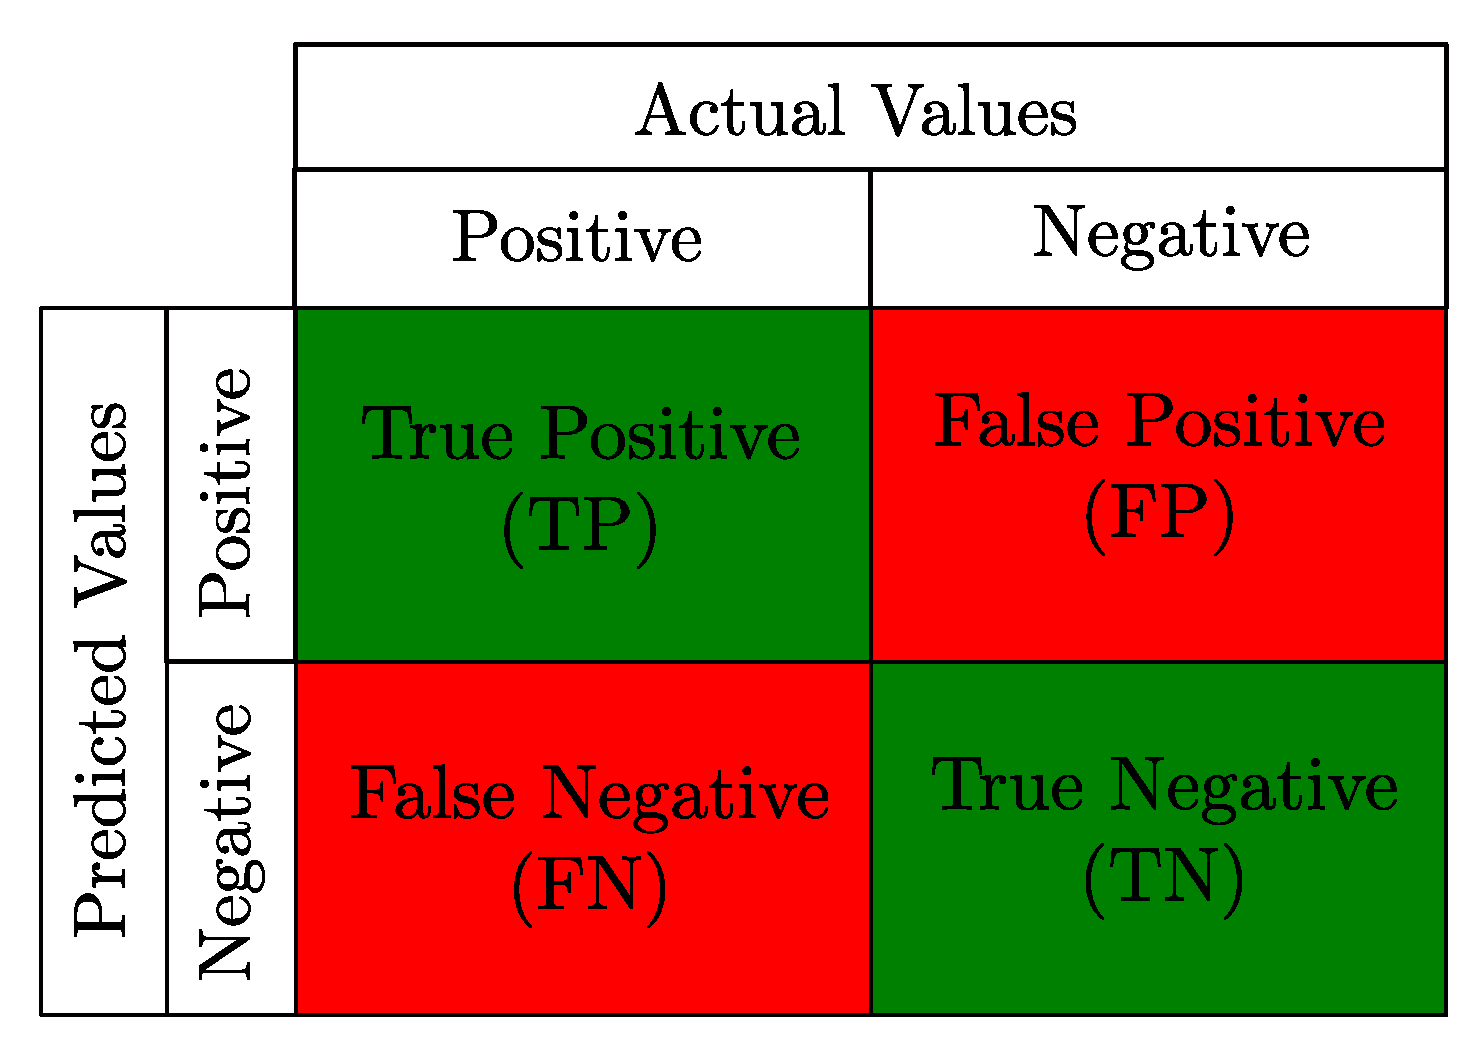
\includegraphics[scale=0.40]{confusion}		
		%\captionsetup{justification=centering}
		\caption{Confusion matrix}
		\label{confusion}
	\end{figure}
	Based on the confusion matrix we can define its entries for the case of keyword extraction as:
	\begin{itemize}
		\item True positives: keywords that are correctly identified by the model.
		\item False positives: non-keywords that are incorrectly identified as keywords by the model.
		\item False negatives: keywords that are not identified by the model
		\item True negatives: non-keywords that are correctly identified as non-keywords by the model (this will not be explicitly calculated). 
	\end{itemize}
	Now we can defined the metrics:
	\begin{itemize}
		\item \textbf{Accuracy} defined as the ratio of correct predictions to the total number of of instances or:
		$$ \text{Accuracy} = \frac{TP + TN}{TP + TN + FP + FN}. $$
		We will not use this measure as it contains the true negatives which do not make sense to calculate for the case of keyword extraction.
		\item \textbf{Precision} is defined as the ratio of true positives to the sum of true positives and false positives or:
		$$ \text{Precision} = \frac{TP}{TP + FP}. $$
		It basically measures the accuracy of the positive predictions made by the model. In terms of keyword extraction, precision measures the fraction of identified keywords that are actually keywords.
		
		\item \textbf{Recall} is defined as the ratio of true positives to the sum of true positives and false negatives or:
		$$ \text{Recall} = \frac{TP}{TP + FN}. $$
		It basically tells us of all the instances that were actually positive, how many the model correctly predicted as positive. In terms of keyword extraction, recall measures the fraction of actual keywords that are correctly identified.
		\item \textbf{F-score} is defined as the harmonic mean of precision and recall or:
		$$ \text{F-score} = \frac{2 \times \text{Precision} \times \text{Recall}}{\text{Precision} + \text{Recall}} $$
		This score tells us how well the model balances between precision and recall. The F-score ranges from $0$ to $1$ and higher scores indicate better performance in both precision and recall.  
	\end{itemize}
	To capture the metrics for all the abstracts, we will average the metrics across all the abstracts, which is also called \textbf{macro-averaging}. We have all the prerequisites, so we can now see the results of keyword extraction on the dataset.
	\newpage
	\subsection{Testing}
	Before discussing the testing results let us address some key elements of keyword extraction:
	\begin{itemize}
		\item All the development and testing were done in Python. The co-occurrence matrix construction was written from scratch. The NLP pipeline was built using the \textit{nltk} library with some specific blocks built from scratch (e.g. the sliding window). The graph and ranking algorithms were built from the \textit{networkx} library. The word embedding "\textit{glove-wiki-gigaword-50}" model \cite{glove} from the \textit{gensim} library was used, with $50$ dimensional vectors.
		\item The human assigned keywords can be subjective and most importantly they can be human generated, so the maximum achievable results when comparing the to the human assigned keywords are less than 100\%.
		\item The expected precision, recall and F-score should be in the range $10 - 40 \%$ as presented in these papers \cite{ying_yan}, \cite{mothe}, \cite{keyword-extraction-0}, \cite{textrank}.
		\item When using the cosine similarity in word embeddings, negative values may arise, and for some of the ranking algorithms we require positive weights (e.g. for path finding). To solve this issue, all the edge weights in a graph were offset by the absolute value of the minimum weight value, so that we only deal with positive values.
		\item To calculate the metrics, we selected the top $n$ keywords calculated by the model, where $n$ is the number of true keywords from the dataset. In such a manner we can directly compare the predicted and true keywords.
	\end{itemize}	
	The final, macro-averaged, results are shown in Table \ref{tab:main_table}. For all the $5000$ papers, the precision, recall and F-score were computed after which they were averaged. The hyperparameter that was changed was the the window size, so for three different values of the window size, we can see the keyword extraction results. 
	
	We can observe that the computed results are in the expected range that other papers have obtained. One unexpected result is that changing the window size didn't have much of an impact on the metrics. The reason for this is the implementation of the sliding window. The sliding window doesn't cross sentences and if sentences are not long, changing the window size will not have much of an impact. Nonetheless, we can observe a slight decrease in performance when increasing window size which was also observed in \cite{textrank}. The explanation is, when using larger window sizes we can capture more context but it might also introduce noise, by including less relevant words, diluting the meaningful co-occurrence patterns, which could lead to a decrease in precision and recall. 
	
	\begin{table}[H] 
		\caption{Keyword extraction results for precision recall and F-score for different window sizes.}
		\label{tab:main_table}
		\hspace*{-1cm}
		\renewcommand\arraystretch{1.1}
		\begin{tabular}{|c|c|>{\centering\arraybackslash}p{3cm}|>{\centering\arraybackslash}p{3cm}|>{\centering\arraybackslash}p{3cm}|}
			\hline
		Window   Size       & Ranking   Algorithm    & Precision (\%) & Recall (\%) & F-score (\%) \\ \Xcline{1-5}{1mm}
		\multirow{5}{*}{3}  & Degree Centrality      & 29.37          & 33.19       & 31.16        \\ \cline{2-5} 
		& Closeness Centrality   & 25.33          & 28.62       & 26.87        \\ \cline{2-5} 
		& Betweenness Centrality & 25.83          & 29.17       & 27.39        \\ \cline{2-5} 
		& Eigenvector Centrality & 27.99          & 31.64       & 29.70        \\ \cline{2-5} 
		& PageRank               & \textbf{29.60}          & \textbf{33.45}       & \textbf{31.40}        \\ \Xcline{1-5}{1mm}
		\multirow{5}{*}{5}  & Degree Centrality      & 29.38          & 33.20       & 31.17        \\ \cline{2-5} 
		& Closeness Centrality   & 24.93          & 28.16       & 26.45        \\ \cline{2-5} 
		& Betweenness Centrality & 25.66          & 28.98       & 27.21        \\ \cline{2-5} 
		& Eigenvector Centrality & 27.93          & 31.57       & 29.63        \\ \cline{2-5} 
		& PageRank               & 29.37          & 33.19       & 31.16        \\ \Xcline{1-5}{1mm}
		\multirow{5}{*}{10} & Degree Centrality      & 28.55          & 32.26       & 30.28        \\ \cline{2-5} 
		& Closeness Centrality   & 24.03          & 27.13       & 25.48        \\ \cline{2-5} 
		& Betweenness Centrality & 25.31          & 28.58       & 26.84        \\ \cline{2-5} 
		& Eigenvector Centrality & 24.34          & 27.49       & 25.81        \\ \cline{2-5} 
		& PageRank               & 28.57          & 32.28       & 30.31        \\ \Xcline{1-5}{1mm}
		\end{tabular}
	\end{table}
	
	The best results were observed for the PageRank ranking algorithm (the TextRank version of it) for the window size of $3$. The low values in precision and recall in no means signify a bad model, as the model correctly found the most important words in the text, but the profound nature of the task is the reason for the values. In regards to the values, having precision and recall in a similar range signifies a balanced performance in terms of correctly identifying true keywords and capturing all true keywords. 
	
	We can also mention the good performance of degree centrality ranking even though it takes only into account the node connections, not the edge weights which indicates the importance of the \textit{distributional hypothesis}.

	\newpage
	\section{Conclusion}
	In this thesis work, we tackled the problem of automatic keyword extraction using graph-based methods and word embeddings. The problem was narrowed down to extract keywords from paper abstracts in the domain of computer science. The foundation of the used approach lays in constructing a graph representation of the co-occurrence relationships among nouns and adjectives within paper abstracts, leveraging the robustness of word embeddings. After building the graph representation of the paper abstracts, various centrality measures for graphs were used to rank the words in the abstract. The measures used were: Degree Centrality, Closeness Centrality, Betweenness Centrality, Eigenvector Centrality and PageRank. Each algorithm brought a perspective to the identification of keywords, offering a nuanced understanding of their importance within the context of the given abstracts.
	
	The evaluation of the model's performance incorporated fundamental metrics such as precision, recall, and F-score. Macro-averaging, accounting for variations in abstract characteristics, provided a comprehensive view of the model's performance. The observed results, falling within the range of outcomes reported in existing literature on this topic, prove the concept of using the ranking algorithms for keyword extraction. The best results were observed for the PageRank algorithm, more specifically the text version of it. 
	
	While the model exhibits promising results, it is essential to acknowledge its limitations. Factors such as domain-specific nuances and the inherent ambiguity of language pose challenges that call for further investigation. Future research endeavors could dive deeper into these challenges, enhancing its adaptability across different datasets.
	
	The most promising features of using a graph-based model, is that it is unsupervised and fast. The swift nature of the model aligns with the practical demands of real-world applications, where efficiency and autonomy are paramount. It most certainly can be used as a particularly good initial guess when doing information retrieval. 
	In conclusion, this thesis highlights the importance of harnessing unsupervised graph-based methods for keyword extraction, providing a scalable and adaptable solution for real-world applications. 
	

	
	
	
	\newpage
	\section{Literature}
	
	\begin{thebibliography}{8}
		\bibitem{word-embedding-survey}
		Almeida, Felipe, and Geraldo Xexéo. "\textit{Word embeddings: A survey}". arXiv preprint arXiv:1901.09069 (2019). \\
		\texttt{URL: }\url{https://arxiv.org/pdf/1901.09069.pdf}
		
		\bibitem{transformers-survey}
		Lin, Tianyang, et al. "\textit{A survey of transformers}". AI Open (2022).\\
		\texttt{URL: }\url{https://www.sciencedirect.com/science/article/pii/S2666651022000146}
		
		\bibitem{great_transformer}
		Luitse, Dieuwertje, and Wiebke Denkena. "\textit{The great transformer: Examining the role of large language models in the political economy of AI}." Big Data \& Society (2021).\\
		\texttt{URL: }\url{https://journals.sagepub.com/doi/pdf/10.1177/20539517211047734}
		
		\bibitem{keyword-extraction-0}
		Zu, Xian, Fei Xie, and Xiaojian Liu. "\textit{Graph-based keyphrase extraction using word and document embeddings}". IEEE International Conference on Knowledge Graph (ICKG) (2020). \\
		\texttt{URL: }\url{https://ieeexplore.ieee.org/abstract/document/9194571}
		
		\bibitem{distributional}
		Sahlgren, Magnus. "\textit{The distributional hypothesis}." Italian Journal of Disability Studies 20 (2008). \\
		\texttt{URL: }\url{https://www.diva-portal.org/smash/get/diva2:1041938/FULLTEXT01.pdf}
		
		\bibitem{stanford_NLP}
		The Stanford NLP Group\\
		\texttt{URL: }\url{https://nlp.stanford.edu/}
		
		\bibitem{tokenizer}
		The nltk Penn Treebank tokenizer. \\
		\texttt{URL: }\url{https://www.nltk.org/api/nltk.tokenize.TreebankWordTokenizer.html}
		
		\bibitem{penn}
		The Penn Treebank. \\
		\texttt{URL: }\url{https://catalog.ldc.upenn.edu/LDC99T42}
		
		\bibitem{pos_tags}
		The nltk PoS tagger. \\
		\texttt{URL: }\url{https://www.nltk.org/api/nltk.tag.pos_tag.html}
		
		\bibitem{lemmatizer}
		Plisson, Joël, Nada Lavrac, and Dunja Mladenic. "\textit{A rule based approach to word lemmatization}." In Proceedings of IS (2004). \\
		\texttt{URL: }\url{https://eprints.um.edu.my/13423/1/rp030_I3007.pdf}
		
		\bibitem{word2vec}
		Word2Vec project information\\
		\texttt{URL: }\url{https://code.google.com/archive/p/word2vec/}
		
		\bibitem{glove}
		GloVe: Global Vectors for Word Representation\\
		\texttt{URL: }\url{https://nlp.stanford.edu/projects/glove/}
		
		\bibitem{multi_sense_we}
		Ruas, T., Grosky, W. and Aizawa, A.  "\textit{Multi-sense embeddings through a word sense disambiguation process}". Expert Systems with Applications,  (2019). \\
		\texttt{URL: }\url{https://arxiv.org/pdf/2101.08700.pdf}
		
		\bibitem{phrase2vec}
		Wu, Yongliang, Shuliang Zhao, and Wenbin Li. "\textit{Phrase2Vec: phrase embedding based on parsing}." Information Sciences (2020). \\
		\texttt{URL: }\url{https://www.sciencedirect.com/science/article/abs/pii/S0020025519311429}
		
		\bibitem{juricGrafovi}
		Jurić Ž. "\textit{Diskretna matematika za studente tehničkih nauka}". ETF Sarajevo, UNSA, (2017). 
		
		\bibitem{networkx_centrality}
		NetworkX Library documentation\\
		\texttt{URL: }\url{https://networkx.org/documentation/stable/reference/algorithms/}
		
		\bibitem{dijkstra}
		Dijkstra, Edsger W. "\textit{A note on two problems in connexion with graphs}." In Edsger Wybe Dijkstra: His Life, Work, and Legacy (2022). \\
		\texttt{URL: }\url{https://hal.science/hal-03171590/document}
		
		\bibitem{bavelas}
		Bavelas, Alex. "\textit{Communication patterns in task‐oriented groups}". The journal of the acoustical society of America (1950). \\
		\texttt{URL: }\url{https://hal.science/hal-03266728/file/bavelas1950groupefmr.pdf}
		
		\bibitem{freeman}
		Freeman, Linton C. "\textit{A set of measures of centrality based on betweenness}". Sociometry (1977). \\
		\texttt{URL: }\url{https://www.jstor.org/stable/3033543?seq=7}
		
		\bibitem{pagerank}
		Brin, Sergey, and Lawrence Page."\textit{The anatomy of a large-scale hypertextual web search engine}". Computer networks and ISDN systems (1998). \\
		\texttt{URL: }\url{https://www.sciencedirect.com/science/article/abs/pii/S016975529800110X}
		
		\bibitem{textrank}
		Mihalcea, Rada, and Paul Tarau. "\textit{Textrank: Bringing order into text}." Proceedings of the 2004 conference on empirical methods in natural language processing (2004). \\
		\texttt{URL: }\url{https://aclanthology.org/W04-3252.pdf}
		
		\bibitem{katz}
		Katz, Leo. "\textit{A new status index derived from sociometric analysis}." Psychometrika (1953). \\
		\texttt{URL: }\url{https://www.cse.cuhk.edu.hk/~cslui/CMSC5734/katz-1953.pdf}
		
		\bibitem{ieeexplore}
		IEEE Xplore digital library.
		\texttt{URL: }\url{https://ieeexplore.ieee.org/search/advanced}
		
		\bibitem{scrapper}
		A script for scraping scientific papers from IEEE Xplore digital Library. \\
		\texttt{URL: }\url{https://github.com/NifulIslam/Multilabel-CS-Keyword-Prediction/tree/master/Scrapper}
		
		\bibitem{dataset}
		The dataset of computer science papers: \\
		\texttt{URL: }\url{https://drive.google.com/drive/folders/1myekdknaLp4KYjUhjOgCLU2DJJoeKs_u?usp=sharing}
		
		\bibitem{ying_yan}
		Ying, Yan, et al. "\textit{A graph-based approach of automatic keyphrase extraction}." Procedia Computer Science (2017).\\
		\texttt{URL: }\url{https://www.sciencedirect.com/science/article/pii/S1877050917303629}
		
		\bibitem{mothe}
		Mothe, J., Ramiandrisoa, F., Rasolomanana, M. "\textit{Automatic keyphrase extraction using graph-based methods}." In Proceedings of the 33rd Annual ACM Symposium on Applied Computing (2018).\\
		\texttt{URL: }\url{https://dl.acm.org/doi/abs/10.1145/3167132.3167392}
		
		
		
		
	\end{thebibliography}

	\end{spacing}
	
\end{document}